\documentclass[a4paper, oneside, notitlepage]{book}
% \documentclass[11pt,twocolumn]{article}
%Use package definitions
\usepackage[margin=1.4in]{geometry}
\usepackage[utf8]{inputenc}
% Load silence package to suppress warnings
\usepackage{silence}
% Suppress warnings related to font shape
\WarningFilter{latexfont}{Font shape `T1/cmbr/m/sc' undefined}
\WarningFilter{latexfont}{Some font shapes were not available, defaults substituted}
%Serif font
\usepackage[T1]{fontenc}
\usepackage{cmbright}
% \usepackage{fouriernc}
\usepackage{textcomp}
\usepackage{amsmath, amssymb, bm}
\usepackage{pdfpages}
%Line through stuff
\usepackage{centernot}
\usepackage{transparent}
\usepackage{varwidth}
%Custom boxes
\usepackage[most]{tcolorbox}
\usepackage{xcolor}
\usepackage{url}
\usepackage{hyperref}
%Algorithm environments
\usepackage{algorithm}
\usepackage{algpseudocode}
%Multiple columns
\usepackage{multicol}
%Tables
\usepackage{array}
\usepackage{booktabs}
%Header
\usepackage{titleps}


\newpagestyle{main}{
\setheadrule{.4pt}% Header rule
\sethead{\sectiontitle}{}{}
% \setfootrule{.4pt}
\setfoot{}{\thepage}{}
}
\pagestyle{main}
% %Space between paragraphs
\setlength{\parskip}{10pt}
%No indentation on the first word of a new paragraph
\setlength{\parindent}{0cm}
%Define where images are stored
\newcommand{\imgpath}{/home/isaac/Documents/Maths/Year_3/LaTeX/Images/}
%Creating a new color box
\newtcolorbox{blackbox}[1][]{colframe=black,colback=white,sharp corners,center,#1}
%Creating the title

%Creating the title
\title{
On the Predictability of the Binance Orderbook 
\author{I.J Lee}
\date{\today}
}


% -----------------------------------------------------------------------
\begin{document}
\maketitle

\begin{center}
   \textbf{Abstract} 
\end{center}
\textbf{TODO}
% In this paper we explore the limit orderbook dynamics of the 
% largest centralized cryptocurrency exchange, namely Binance.
% We take an exploratory approach, aiming to assess the information content
% and predictive power of information contained in the limit orderbook.

\clearpage
\tableofcontents

\chapter{Introduction}
\hrule
\vspace{40pt}

\section{Contribution}
\textbf{TODO}

\section{Related Works}
\textbf{TODO}

\section{The Orderbook}
On centralized exchanges, \textit{the orderbook} is the main data structure used to
organize buying and selling activity. 

There are two main orders a client can submit, \textit{market orders} and \textit{limit orders}.
Market orders get instantly matched at the \textit{best available price}
and executed. Limit orders specify a desired transaction price to buy/sell for a given volume.
If the order cannot be instantly filled by current supply, the limit order will
be posted to the limit orderbook, to be filled by future matching orders.
Essentially the orderbook keeps track of the current (unfilled) supply and demand.
The limit orders that are posted to the orderbook are organized into levels,
indexed by price. So all limit orders with the same price (and side) are 
combined into a single level, and their volumes are aggregated.

Note that the orderbook can contain hundreds of thousands of levels but the majority
of the activity is focused around the top levels.

The \textit{bids} are the buy orders, and the \textit{asks}
are the sell orders. Ask levels are sorted by price in ascending order and 
bid levels are sorted in descending order. The first/top ask level price is the
lowest ask price, and the first/top bid level price is the highest bid price. 
So if a client wishes to buy, the \textit{best available price} is the first/top/lowest ask price
and if they wish to sell, their best available price is first/top/highest bid price.

See figure \ref{fig:orderbook} for a visual representation of the limit orderbook.

When new orders arrive, they will be matched against the orderbook and either posted or filled.
If enough orders are matched at a certain price, all the volume for that price level 
will be consumed and the price will be removed from the orderbook and the next best price will take its place for that level.

In this way, the state of the orderbook is constantly changing, as new orders are submitted
and price levels are partially or fully filled.

We define the mid price to be the average of the best bid and ask price.
This single value is often used to represent the current price of the asset.

We also define the spread to be the difference between the best bid and ask price.
Smaller spreads are highly correlated with high trade volume \cite{ARITRA2021}.

\begin{figure}[htpb]
    \centering
    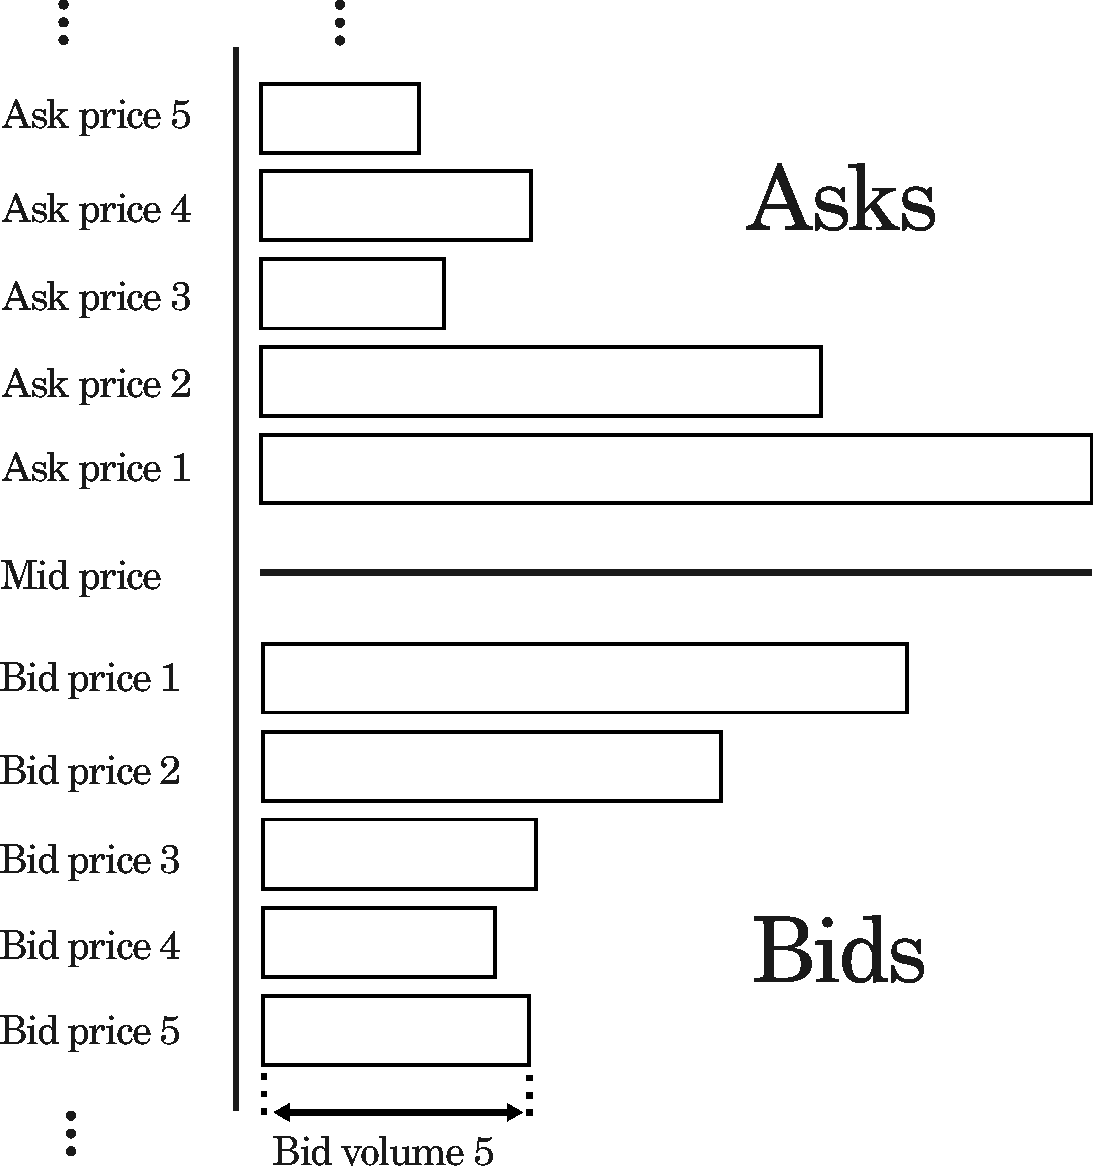
\includegraphics[width=0.5\textwidth]{./images/orderbook.pdf}
    \caption{A visual representation of the orderbook. (Specifically for L2 data).}
    \label{fig:orderbook}
\end{figure}

It is important to note that there are three main levels of granularity 
when it comes to orderbook representations.
Firstly we have L1 data, which is only the best bids and asks, with their corresponding volumes.
Then we have L2 data, which is all price levels with their corresponding volumes, with one volume value
per price level. (I.e volumes are summed across orders for each price level). Then the most granular is L3 data,
which contains all price levels, with multiple volume values for each price level. Specifically the volumes at a given price
level are broken down into their individual order values. So if, from time $t-1$ to time $t$, 2 orders
are submitted with volumes $v_a$ and $v_b$, then the $L2$ representation would show $V_t = V_{t-1} + v_a + v_b$,
whereas the L3 representation would give us  $\bm{V_t} = [\bm{V_{t-1}}; v_a, v_b]$

For a more in depth exposition of the mechanism of the limit orderbook, we refer the interested reader to \cite{MARTIN2013}.


\section{The Data}
In this section we introduce our data source and give some visualizations.

\subsection{Data Source}

Our data has been gathered from Binance directly.

Binance is the largest cryptocurrency exchange in terms of daily volume, with a revenue of \$12 billion in 2022 according to \cite{TULLY2023}. 
It was founded in 2017 by Changpeng Zhao. %Binance was initially based in China, then moved to Japan shortly before the Chinese government restricted cryptocurrency companies. Binance then left Japan for Malta and currently has no official company headquarters. 

Binance was chosen because of its high volume, popularity and decent API availability.
Binance also offers USDT futures which is the main security of focus for this paper.

\section{Websocket Data}
Binance offers live Websocket data with various endpoints. 
We use the endpoint: \begin{verbatim}wss://fstream.binance.com/ws/{symbol}@depth{L}@100ms\end{verbatim} 
to stream top L best bids and asks every approximately 100ms.
We log this data to an SQL database on an AWS server.

Due to free-tier limitations we only have about 30GB of storage on the server,
which corresponds to approximately a month of data for four symbols. 
This is also about the limit of how much data we can fit into memory at any one time. For these reasons
we only work with one month of data, from the start to the end of February, 2024.

Since we are looking at such high frequencies, this data should be satisfactory.

We choose BTCUSDT, ETHUSDT, SOLUSDT and MATICUSDT as our symbols of interest. We choose
these because they are all high enough volume to have good liquidity but also have significant
enough difference in traded volume so that their comparative study should be interesting.

We store this data as a DataFrame for each symbol. Each row contains the top 10 bid and ask prices and quantities
for a given time. See Table \ref{table:websocket} for an example DataFrame for MATICUSDT. 

\begin{table*}[ht]
\centering
\resizebox{\textwidth}{!}{
    \begin{tabular}{|c|c|c|c|c|c|c|c|c|c|c|c|c|c|}
    \hline
    Row & timestamp & ask\_price\_1 & ... & ask\_price\_10 & bid\_price\_1 & ... & bid\_price\_10 & ask\_qty\_1 & ... & ask\_qty\_10 & bid\_qty\_1 & ... & bid\_qty\_10 \\
    \hline
    0 & 1707138494390 & 0.7877 & ... & 0.7886 & 0.7876 & ... & 0.7867 & 9368.0 & ... & 58006.0 & 15095.0 & ... & 44990.0 \\
    1 & 1707138494515 & 0.7877 & ... & 0.7886 & 0.7876 & ... & 0.7867 & 9367.0 & ... & 58006.0 & 15095.0 & ... & 84785.0 \\
    2 & 1707138494760 & 0.7877 & ... & 0.7886 & 0.7876 & ... & 0.7867 & 9367.0 & ... & 58006.0 & 15095.0 & ... & 44990.0 \\
    3 & 1707138494881 & 0.7877 & ... & 0.7886 & 0.7876 & ... & 0.7867 & 9367.0 & ... & 58006.0 & 15095.0 & ... & 44990.0 \\
    4 & 1707138495248 & 0.7877 & ... & 0.7886 & 0.7876 & ... & 0.7867 & 9356.0 & ... & 58006.0 & 15099.0 & ... & 44990.0 \\
    \vdots & \vdots & \vdots & \vdots & \vdots & \vdots & \vdots & \vdots & \vdots & \vdots & \vdots & \vdots & \vdots & \vdots \\
    11294483 & 1708857980137 & 0.9726 & ... & 0.9735 & 0.9725 & ... & 0.9716 & 16199.0 & ... & 64495.0 & 20555.0 & ... & 37554.0 \\
    11294484 & 1708857980246 & 0.9726 & ... & 0.9735 & 0.9725 & ... & 0.9716 & 16199.0 & ... & 61163.0 & 19527.0 & ... & 37554.0 \\
    11294485 & 1708857980360 & 0.9726 & ... & 0.9735 & 0.9725 & ... & 0.9716 & 20199.0 & ... & 61163.0 & 19527.0 & ... & 37554.0 \\
    11294486 & 1708857980494 & 0.9726 & ... & 0.9735 & 0.9725 & ... & 0.9716 & 21610.0 & ... & 61163.0 & 19577.0 & ... & 37554.0 \\
    11294487 & 1708857980602 & 0.9726 & ... & 0.9735 & 0.9725 & ... & 0.9716 & 22992.0 & ... & 61163.0 & 18401.0 & ... & 37554.0 \\
    \hline
    \end{tabular}
}
\caption{Example data for MATICUSDT}
\label{table:websocket}
\end{table*}

We note that the websocket data is not regular, but comes \textbf{approximately} every 100ms.
This means that the time delta between updates is not constant and therefore this is technically not
a timeseries in the proper sense. For some of our applications we will resample this data into regular intervals.

\textbf{TODO:} Latency analysis.


\section{A Visual Exploration}

We define the height of a level $\ell \in \{ 1, 2, \dots, 10 \}$ on the $x$ side as $\Delta p_{\ell}^x = p_{\ell}^x - p_{\ell-1}^x$, with $x \in{\{ B,A \}}$. 
Where $B,A$ denote the bid, ask sides respectively. 
In other words, the price difference between the the $\ell^{th}$ and $\ell-1^{th}$ bid/ask price level.
We note that by definition, $\Delta p_{\ell}^A < 0, ~ ~ \forall \ell$ and $\Delta p_{\ell}^B > 0, ~ ~ \forall \ell$

The length of a level $\ell$ on the $x$ side is denoted by $q^x_{\ell}$ and represents the total volume
for the $\ell^{th}$ price level.

We also define the mid price as an average of the best bid and ask price, i.e

\begin{equation}
    p_0 := \frac{1}{2} (p^A_{1} + p^B_{1}) \label{mid}
\end{equation}

Following \cite{CAO2009}, we normalize the level heights by the price difference
between the 10th level and the mid price, i.e total height. 
The level length is also normalized by the total length from the first level to the 10th level.
I.e 

\begin{align}
    \tilde{q}_{l}^x &:= \frac{q_{l}^x}{\sum_{j=1}^{10} q_{j}^x}  \\
    \Delta\tilde{p}_{l}^x &:= \frac{\Delta p_{l}^x}{\sum_{j=1}^{10} \Delta p_{j}^x} = \frac{\Delta p_{l}^x}{|p_{0} - p_{10}^x|}
\end{align}

We average the bids and asks over all entries and then calculate the normalized lengths
and heights. We visualize the results for each symbol in Figure \ref{shape}.
This gives us a good idea of the overall average shape of the orderbooks.

We see that across all symbols the average orderbook is mostly symmetric,
which is what we would expect. Perhaps more interestingly we see that for BTCUSDT the relative
length for the first price level is much larger (higher volume) compared to the other top 10 levels.
In fact, we observe that the relative length of the first level seems to be increasing as a function
of the symbols popularity/volume. If we were to order the symbols in terms of trading volume, from 
lowest to highest we would have MATICUSDT, SOLUSDT, ETHUSDT and BTCUSDT. This ordering
is also the ordering of the relative length of the first level. So it seems that
the more popular a symbol is, the more the volume is weighted towards the top of
the orderbook. Also another interesting point is that after the first level
the relative lengths are almost identical, suggesting e.g that there is just as much
activity in the 10th level compared to the 2nd level of the orderbooks.

\cite{CAO2009} used a similar methodology to visualize the shape of the orderbook,
but for stocks from the Australian Securities Exchange, ASX. The shape of the orderbook
found in \cite{CAO2009} looks a lot like the MATICUSDT orderbook shape, which
agrees with our previously discussed first level length - volume relationship, since the ASX
(in 2009) had much less volume compared to BTCUSDT in 2024.

\begin{figure}[htpb]
    \centering
    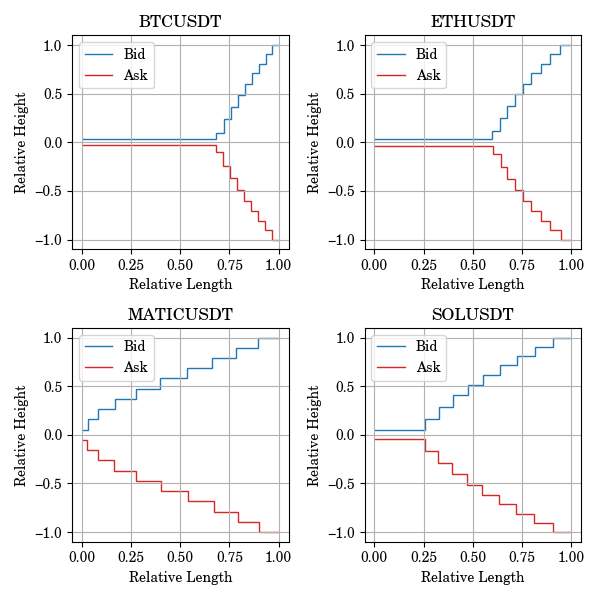
\includegraphics[width=1.0\textwidth]{./images/shapes.png}
    \caption{Orderbook normalized average heights and lengths for each symbol. \textbf{TODO:} Re-plot these stacked.}
    \label{shape}
\end{figure}






\chapter{Price Impact}
% \section{The Modelling Objective}
% Recall previously we defined the mid price (which we will now denote as $p$) as the the average of the best bid and best ask.
% This will be our target variable in this chapter. The quantity we wish to predict.
%
% One could frame this as a regression problem, directly predicting the mid price value
% at some future time, however due to the low signal to noise ratio in our data, and non-stationarity of the mid price, this is perhaps not the best approach. 
% Instead we will convert this to a classification problem, by predicting the sign of the mid price returns over some future horizon.
%
% \begin{figure}[htpb]
%     \centering
%     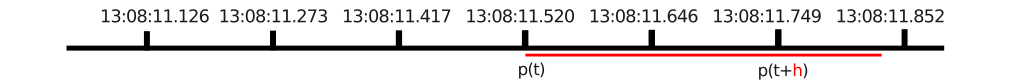
\includegraphics[width=1.0\textwidth]{./images/timeline.png}
%     \caption{Visual demonstration of lookahead price, with irregularly spaced data.}
% \end{figure}
%
% More concretely, at time $t$, if we define the future returns as:
% \[
%     R(t+h) := \frac{p(t+h) - p(t)}{p(t)}
% .\]
%
% then our label at time $t$ is given by:
% \begin{equation}
%     y_t :=  \begin{cases}
%         1 & \text{if } R(t+h) > \epsilon\\
%         0 & \text{if } R(t+h) \in [-\epsilon, \epsilon]\\
%         -1 & \text{if } R(t+h) < -\epsilon
%     \end{cases}
%     \label{equation:modelling_objective}
% \end{equation}
%
% Where $\epsilon$ is a hyperparameter that we can adjust.
%
% So our modeling objective is to predict each $y_t$, given the information up to and including time $t$.
%
% \section{Linear Models}
% Before moving onto more complex models, we start with some simple robust linear models.
%
In this chapter we follow the work of \cite{CONT2013} and model the linear price
impact of orderbook events.

\section{Orderflow Imbalance}

We start by defining the Orderflow Imbalance, a stationary transformation of the orderbook data
first introduced in \cite{CONT2013}.

Since mid price movement is governed by supply and demand, we need to identify
the different orderbook states and how they relate to supply and demand.
We will initially only concern ourselves with the top of the orderbook.

For each of our observations, we have the best bid price and best bid quantity,
which we denote by $p^B, q^B$ and the best ask price and best ask quantity  $p^A, q^A$.
If we enumerate our observations by $n$, then according to \cite{CONT2013}, we have
the following orderbook events:
 \begin{itemize}
     \item $p_n^B > p_{n-1}^B$ or  $q_n^B > q_{n-1}^B$, suggesting an increase in demand.
     \item $p_n^B < p_{n-1}^B$ or  $q_n^B < q_{n-1}^B$, suggesting a decrease in demand.
     \item $p_n^A < p_{n-1}^A$ or  $q_n^A > q_{n-1}^A$, suggesting an increase in supply.
     \item $p_n^A > p_{n-1}^A$ or  $q_n^A < q_{n-1}^A$, suggesting a decrease in supply.
\end{itemize}
Then \cite{CONT2013} define the quantity $e_n$ to represent the contribution of the  $n^{\text{th}}$ event
as $e_n = e_n^B - e_n^A$ where  $e_n^B$ and $e_n^A$ are defined in (\ref{eBeA}).
\begin{equation}
    \begin{aligned}
        e_{n}^B &:= I_{\{ p_{n}^B \geq p_{n-1}^B \}} q_{n}^B  - I_{\{ p_{n}^B \leq p_{n-1}^B \}} q_{n-1}^B \\
        e_{n}^A &:= I_{\{ p_{n}^A \leq p_{n-1}^A \}} q_{n}^A - I_{\{ p_{n}^A \geq p_{n-1}^A \}} q_{n-1}^A
    \end{aligned}
    \label{eBeA}
\end{equation}
% &= (\Delta q_{n}^B I_{\{ \Delta p_{n}^B \leq 0 \}} + q_{n}^B (I_{\{ \Delta p_{n}^B \geq 0 \}}  - I_{\{ \Delta p_{n}^B \leq 0 \}})) - (\Delta q_{n}^A I_{\{ \Delta p_{n}^A \geq 0 \}} + q_{n}^A (I_{\{ \Delta p_{n}^A \leq 0 \}} - I_{\{ \Delta p_{n}^A \geq 0\}})) \label{diff}
% Where (\ref{diff}) allows for efficient computation using the diff operator.
Then we sum these individual contributions from time $t-h$ to the current time $t$,
to get the Order Flow Imbalance at time $t$:
\begin{equation}
    \text{OFI}_h(t) := \sum_{n : t_n \in [t-h, t]} e_n
    \label{OFI}
\end{equation}

\section{Linear Price Impact Model}
\textbf{TODO: Add more detail in this section}

Firstly, let us define $\Delta p_{\delta}(t+h) := (p(t+h) - p(t)) / \delta$ i.e the change in price
measured in ticks, where $\delta$ is the ticksize for the given symbol. Using the Binance API we
retrieve the ticksizes as:  % TODO: Format this better
\begin{table}[ht]
    \centering
    \begin{tabular}{|l|l|}
        \hline
        \textbf{Symbol} & \textbf{$\delta$} \\
        \hline
        BTCUSDT & 0.1 \\
        \hline
        ETHUSDT & 0.01 \\
        \hline
        SOLUSDT & 0.001 \\
        \hline
        MATICUSDT & 0.0001 \\
        \hline
    \end{tabular}
    \caption{Symbols and their ticksizes, $\delta$.}
\end{table}


Then \cite{CONT2013} suggest the following relation:
\begin{equation}
    \Delta p_{\delta}(t) = \beta \text{OFI}_h(t) + \epsilon_t \label{linearrelation}
\end{equation}
where $\beta$ is the \textit{price impact coefficient} and $\epsilon_t$ is the noise
term. So $\beta$ measures the instantaneous impact of the $n^{th}$ event on the mid price. 

\cite{CONT2013} assume the price impact coefficients are constant for half-hour intervals (indexed by $i$),
and estimate them using OLS:
\begin{equation}
    \Delta p_{\delta}(t) = \hat{\beta}_i \text{OFI}_h(t) + \hat{\alpha}_i + \hat{\epsilon}_t
\end{equation}


\section{PanelOLS Results}
We split our data into half-hour windows and then perform PanelOLS across windows
to estimate the average coefficients.


We start with $h = 1000ms$.
\clearpage

\begin{table}[htbp!]
\textbf{BTCUSDT PanelOLS Results for h = 1000ms}
\begin{center}
\begin{tabular}{lclc}
\hline
\textbf{Dep. Variable:}    &         $\Delta p_{\delta}$         & \textbf{  R-squared:         }   &      0.3590      \\
\textbf{Estimator:}        &      PanelOLS      & \textbf{  R-squared (Between):}  &     -0.3865      \\
\textbf{No. Observations:} &      12891080      & \textbf{  R-squared (Within):}   &      0.3590      \\
\textbf{Date:}             &  Tue, Mar 26 2024  & \textbf{  R-squared (Overall):}  &      0.3585      \\
\textbf{Time:}             &      16:15:04      & \textbf{  Log-likelihood     }   &    -6.11e+07     \\
\textbf{Cov. Estimator:}   &     Clustered      & \textbf{                     }   &                  \\
\textbf{}                  &                    & \textbf{  F-statistic:       }   &    7.218e+06     \\
\textbf{Entities:}         &        956         & \textbf{  P-value            }   &      0.0000      \\
\textbf{Avg Obs:}          &     1.348e+04      & \textbf{  Distribution:      }   &  F(1,12890123)   \\
\textbf{Min Obs:}          &       953.00       & \textbf{                     }   &                  \\
\textbf{Max Obs:}          &     1.676e+04      & \textbf{  F-statistic (robust):} &      4743.2      \\
\textbf{}                  &                    & \textbf{  P-value            }   &      0.0000      \\
\textbf{Time periods:}     &       16761        & \textbf{  Distribution:      }   &  F(1,12890123)   \\
\textbf{Avg Obs:}          &       769.11       & \textbf{                     }   &                  \\
\textbf{Min Obs:}          &       1.0000       & \textbf{                     }   &                  \\
\textbf{Max Obs:}          &       956.00       & \textbf{                     }   &                  \\
\textbf{}                  &                    & \textbf{                     }   &                  \\
\hline
\end{tabular}
\begin{tabular}{lcccccc}
             & \textbf{Parameter} & \textbf{Std. Err.} & \textbf{T-stat} & \textbf{P-value} & \textbf{Lower CI} & \textbf{Upper CI}  \\
\hline
\textbf{OFI} &       1.1829       &       0.0172       &      68.871     &      0.0000      &       1.1492      &       1.2166       \\
\hline
\end{tabular}
%\caption{PanelOLS Estimation Summary}
\end{center}
F-test for Poolability: 19.309, \\
P-value: 0.0000, \\ 
Distribution: F(955,12890123),\\
Included effects: Entity.
\end{table}

\begin{figure}[htpb!]
    \centering
    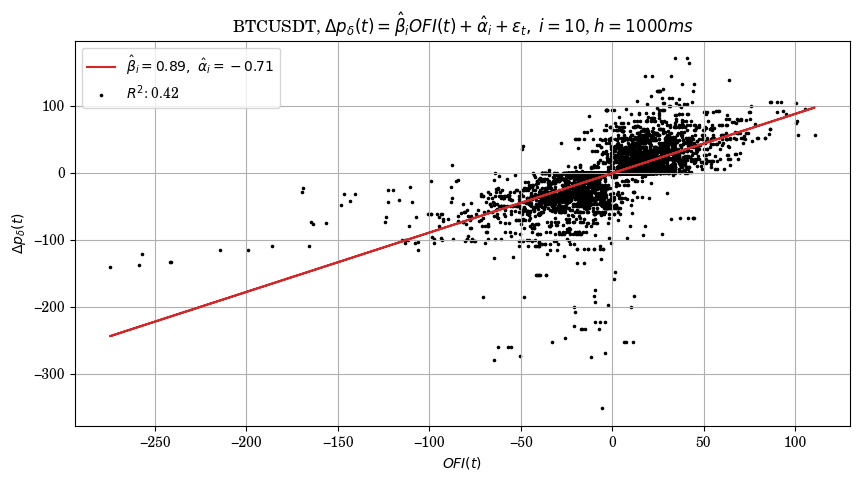
\includegraphics[width=0.8\textwidth]{./images/btcusdt_h=1000ms_contemp_OFI.png}
    \caption{OFI contemporaneous regression for an example half-hour window for BTCUSDT.}
    \label{fig:contemp_OFI_btcusdt}
\end{figure}

\clearpage




\begin{table*}
\textbf{ETHUSDT PanelOLS Results for h = 1000ms}
\begin{center}
\begin{tabular}{lclc}
\hline
\textbf{Dep. Variable:}    &         $\Delta p_{\delta}$         & \textbf{  R-squared:         }   &      0.3407      \\
\textbf{Estimator:}        &      PanelOLS      & \textbf{  R-squared (Between):}  &     -0.5821      \\
\textbf{No. Observations:} &      13612890      & \textbf{  R-squared (Within):}   &      0.3407      \\
\textbf{Date:}             &  Tue, Mar 26 2024  & \textbf{  R-squared (Overall):}  &      0.3401      \\
\textbf{Time:}             &      16:18:43      & \textbf{  Log-likelihood     }   &    -5.922e+07    \\
\textbf{Cov. Estimator:}   &     Clustered      & \textbf{                     }   &                  \\
\textbf{}                  &                    & \textbf{  F-statistic:       }   &    7.034e+06     \\
\textbf{Entities:}         &        956         & \textbf{  P-value            }   &      0.0000      \\
\textbf{Avg Obs:}          &     1.424e+04      & \textbf{  Distribution:      }   &  F(1,13611933)   \\
\textbf{Min Obs:}          &     1.058e+04      & \textbf{                     }   &                  \\
\textbf{Max Obs:}          &     1.654e+04      & \textbf{  F-statistic (robust):} &      4554.0      \\
\textbf{}                  &                    & \textbf{  P-value            }   &      0.0000      \\
\textbf{Time periods:}     &       16538        & \textbf{  Distribution:      }   &  F(1,13611933)   \\
\textbf{Avg Obs:}          &       823.13       & \textbf{                     }   &                  \\
\textbf{Min Obs:}          &       1.0000       & \textbf{                     }   &                  \\
\textbf{Max Obs:}          &       956.00       & \textbf{                     }   &                  \\
\textbf{}                  &                    & \textbf{                     }   &                  \\
\hline
\end{tabular}
\begin{tabular}{lcccccc}
             & \textbf{Parameter} & \textbf{Std. Err.} & \textbf{T-stat} & \textbf{P-value} & \textbf{Lower CI} & \textbf{Upper CI}  \\
\hline
\textbf{OFI} &       0.0891       &       0.0013       &      67.483     &      0.0000      &       0.0866      &       0.0917       \\
\hline
\end{tabular}
%\caption{PanelOLS Estimation Summary}
\end{center}
F-test for Poolability: 21.726, \\
P-value: 0.0000, \\
Distribution: F(955,13611933), \\
Included effects: Entity.
\end{table*}

\begin{figure*}[htpb]
    \centering
    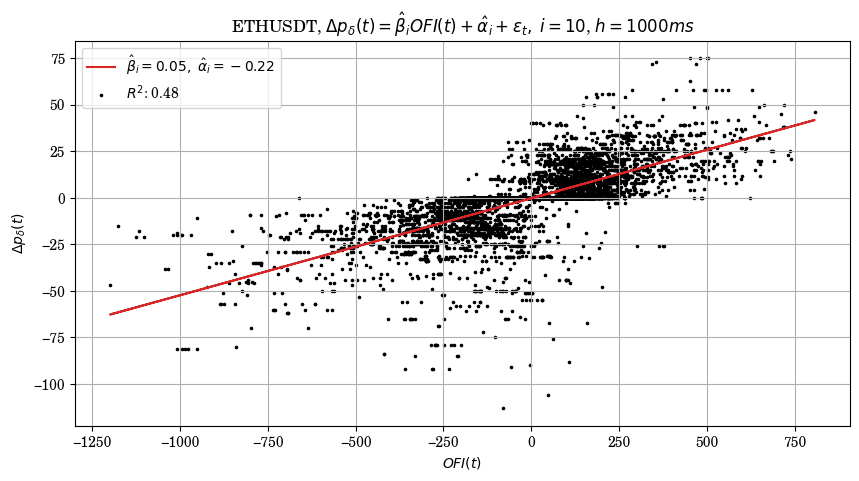
\includegraphics[width=0.8\textwidth]{./images/ethusdt_h=1000ms_contemp_OFI.png}
    \caption{OFI contemporaneous regression for an example half-hour window for ETHUSDT.}
\end{figure*}
\clearpage




\begin{table*}
\textbf{SOLUSDT PanelOLS Results for h = 1000ms}
\begin{center}
\begin{tabular}{lclc}
\hline
\textbf{Dep. Variable:}    &         $\Delta p_{\delta}$         & \textbf{  R-squared:         }   &      0.2828      \\
\textbf{Estimator:}        &      PanelOLS      & \textbf{  R-squared (Between):}  &     -0.3992      \\
\textbf{No. Observations:} &      13334051      & \textbf{  R-squared (Within):}   &      0.2828      \\
\textbf{Date:}             &  Tue, Mar 26 2024  & \textbf{  R-squared (Overall):}  &      0.2824      \\
\textbf{Time:}             &      16:21:12      & \textbf{  Log-likelihood     }   &    -5.176e+07    \\
\textbf{Cov. Estimator:}   &     Clustered      & \textbf{                     }   &                  \\
\textbf{}                  &                    & \textbf{  F-statistic:       }   &    5.258e+06     \\
\textbf{Entities:}         &        957         & \textbf{  P-value            }   &      0.0000      \\
\textbf{Avg Obs:}          &     1.393e+04      & \textbf{  Distribution:      }   &  F(1,13333093)   \\
\textbf{Min Obs:}          &       7478.0       & \textbf{                     }   &                  \\
\textbf{Max Obs:}          &     1.647e+04      & \textbf{  F-statistic (robust):} &      428.29      \\
\textbf{}                  &                    & \textbf{  P-value            }   &      0.0000      \\
\textbf{Time periods:}     &       16473        & \textbf{  Distribution:      }   &  F(1,13333093)   \\
\textbf{Avg Obs:}          &       809.45       & \textbf{                     }   &                  \\
\textbf{Min Obs:}          &       1.0000       & \textbf{                     }   &                  \\
\textbf{Max Obs:}          &       957.00       & \textbf{                     }   &                  \\
\textbf{}                  &                    & \textbf{                     }   &                  \\
\hline
\end{tabular}
\begin{tabular}{lcccccc}
             & \textbf{Parameter} & \textbf{Std. Err.} & \textbf{T-stat} & \textbf{P-value} & \textbf{Lower CI} & \textbf{Upper CI}  \\
\hline
\textbf{OFI} &       0.0128       &       0.0006       &      20.695     &      0.0000      &       0.0116      &       0.0140       \\
\hline
\end{tabular}
%\caption{PanelOLS Estimation Summary}
\end{center}
F-test for Poolability: 15.871, \\
P-value: 0.0000, \\
Distribution: F(956,13333093), \\
Included effects: Entity.
\end{table*}

\begin{figure*}[htpb]
    \centering
    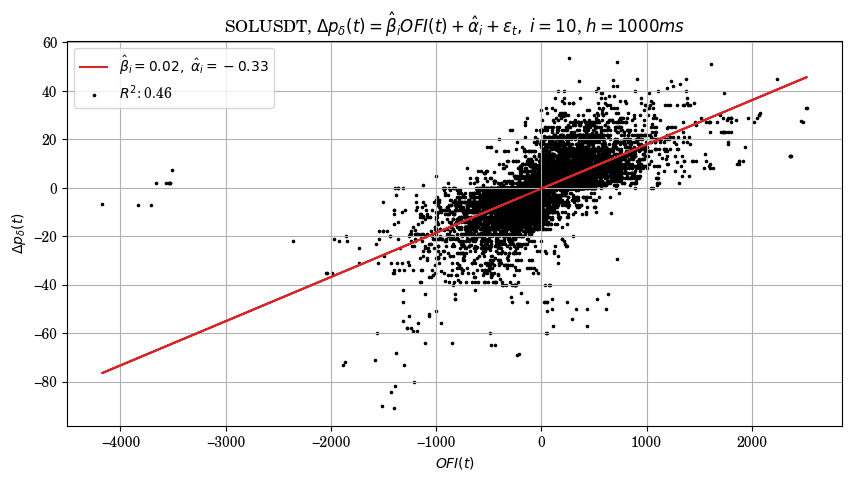
\includegraphics[width=0.8\textwidth]{./images/solusdt_h=1000ms_contemp_OFI.png}
    \caption{OFI contemporaneous regression for an example half-hour window for SOLUSDT.}
\end{figure*}

\clearpage




\begin{table*}
\textbf{MATICUSDT PanelOLS Results for h = 1000ms}
\begin{center}
\begin{tabular}{lclc}
\hline
\textbf{Dep. Variable:}    &         $\Delta p_{\delta}$         & \textbf{  R-squared:         }   &      0.4133      \\
\textbf{Estimator:}        &      PanelOLS      & \textbf{  R-squared (Between):}  &     -0.0188      \\
\textbf{No. Observations:} &      11294487      & \textbf{  R-squared (Within):}   &      0.4133      \\
\textbf{Date:}             &  Tue, Mar 26 2024  & \textbf{  R-squared (Overall):}  &      0.4130      \\
\textbf{Time:}             &      16:23:26      & \textbf{  Log-likelihood     }   &    -1.58e+07     \\
\textbf{Cov. Estimator:}   &     Clustered      & \textbf{                     }   &                  \\
\textbf{}                  &                    & \textbf{  F-statistic:       }   &    7.955e+06     \\
\textbf{Entities:}         &        956         & \textbf{  P-value            }   &      0.0000      \\
\textbf{Avg Obs:}          &     1.181e+04      & \textbf{  Distribution:      }   &  F(1,11293530)   \\
\textbf{Min Obs:}          &       5754.0       & \textbf{                     }   &                  \\
\textbf{Max Obs:}          &     1.639e+04      & \textbf{  F-statistic (robust):} &      2882.6      \\
\textbf{}                  &                    & \textbf{  P-value            }   &      0.0000      \\
\textbf{Time periods:}     &       16388        & \textbf{  Distribution:      }   &  F(1,11293530)   \\
\textbf{Avg Obs:}          &       689.19       & \textbf{                     }   &                  \\
\textbf{Min Obs:}          &       1.0000       & \textbf{                     }   &                  \\
\textbf{Max Obs:}          &       956.00       & \textbf{                     }   &                  \\
\textbf{}                  &                    & \textbf{                     }   &                  \\
\hline
\end{tabular}
\begin{tabular}{lcccccc}
             & \textbf{Parameter} & \textbf{Std. Err.} & \textbf{T-stat} & \textbf{P-value} & \textbf{Lower CI} & \textbf{Upper CI}  \\
\hline
\textbf{OFI} &     3.108e-05      &     5.789e-07      &      53.690     &      0.0000      &     2.995e-05     &     3.222e-05      \\
\hline
\end{tabular}
%\caption{PanelOLS Estimation Summary}
\end{center}
F-test for Poolability: 15.992, \\
P-value: 0.0000, \\
Distribution: F(955,11293530), \\
Included effects: Entity.
\end{table*}

\begin{figure*}[htpb]
    \centering
    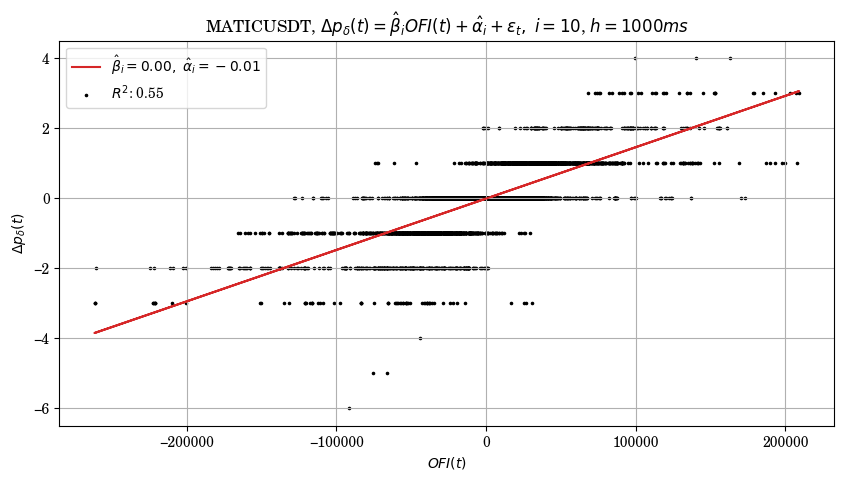
\includegraphics[width=0.8\textwidth]{./images/maticusdt_h=1000ms_contemp_OFI.png}
    \caption{OFI contemporaneous regression for an example half-hour window for MATICUSDT.}
    \label{fig:contemp_OFI_maticusdt}
\end{figure*}

\clearpage

So we observe very similar $R^2$ values across all symbols, around $0.35$, confirming the
linear relation (\ref{linearrelation}). %Interestingly we see that the pooled $\hat{\beta}$ coefficients
% are all orders of magnitude different from each other. This is due to the fact that, whilst order flow
% imbalance is stationary, it is not directly comparable across symbols, since it relies
% on quantity traded, which can vary significantly across symbols.

In figures \ref{fig:contemp_OFI_btcusdt} - \ref{fig:contemp_OFI_maticusdt} 
we also visually examine a half-hour window for each symbol.

So very interestingly we see that the $\Delta p_{\delta}(t)$ values for MATICUSDT
are far more sparse than the other symbols, with fewer unique values, and much more clearly
defined steps. This is much more similar to the results of \cite{CONT2013} and 
perhaps is characteristic of securities with lower volume.

We repeat the procedure for different values of $h$ and plot the results in figure \ref{r2_h}.
We see that $R^2$ increases in  $h$ and then plateaus around $h=20,000ms$.

Instead of averaging across intervals, we can also examine how the price impact coefficients change
across intervals. We visualize the results in figures \ref{fig:BTCUSDT_beta_across_time} - \ref{fig:MATICUSDT_beta_across_time}.
We see that for our data, for all symbols the average price impact coefficient is initially decreasing in time
for the first few hours of the day. It then recovers and begins to (roughly) increase again.
We also see that the variance of the price impact coefficients are fairly constant across different intervals.

The fact that we have trends in price impact coefficients, suggests that
the impact of a new orderbook event on the mid price varies throughout the day, with
some periods having less impact. (Assuming the linear price impact model given by (\ref{linearrelation})).
The smallest average coefficients seem to occur around 06:00AM and so we suggest placing trades around this time
if the goal is to minimize price impact.

\begin{figure*}[htpb]
   \centering
   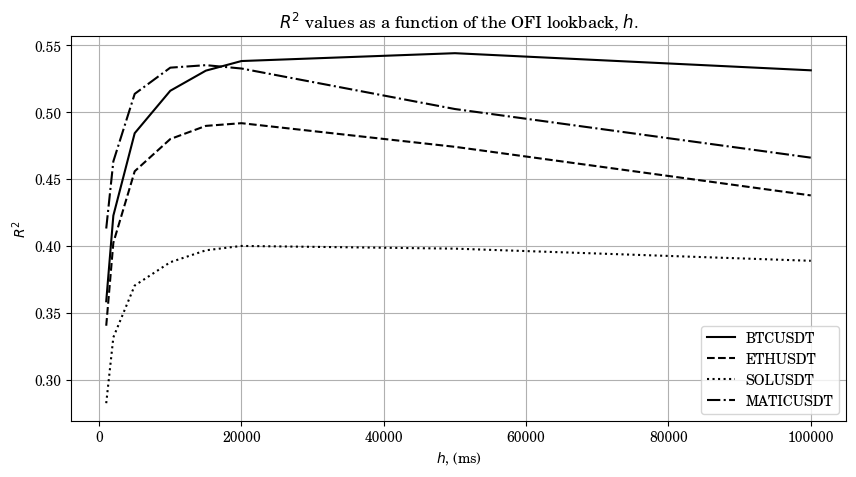
\includegraphics[width=1.0\textwidth]{./images/OFI_r2_h.png}
   \caption{Effect on contemporaneous regression $\Delta p_{\delta}(t) = \hat{\beta}_i \text{OFI}_h(t) + \hat{\alpha}_i + \hat{\epsilon}_t$,
       $R^2$ values when varying the lookback period that defines $\text{OFI}_h(t)$.
    }
   \label{r2_h}
\end{figure*}

\begin{figure*}[htpb]
    \centering
    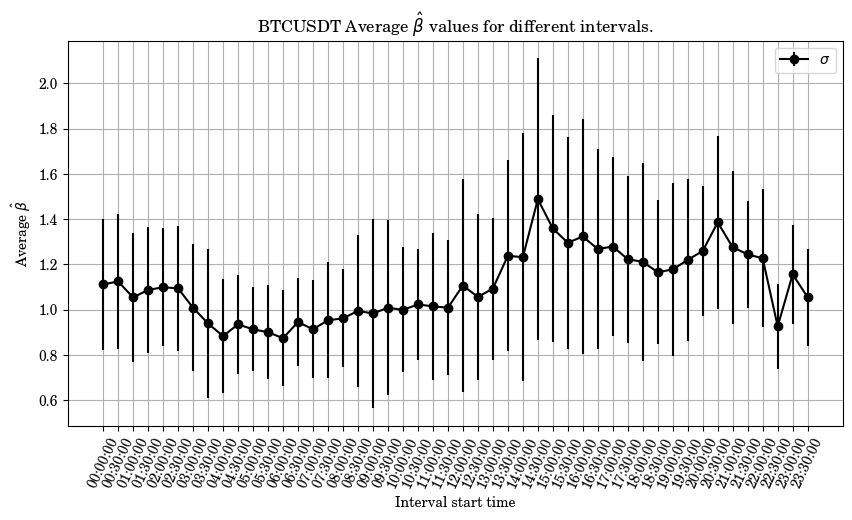
\includegraphics[width=0.8\textwidth]{./images/BTCUSDT_beta_across_time.png}
    \caption{BTCUSDT Average price impact coefficients for different half-hour intervals. Note that errorbars represent standard deviations.}
    \label{fig:BTCUSDT_beta_across_time}
\end{figure*}


\begin{figure*}[htpb]
    \centering
    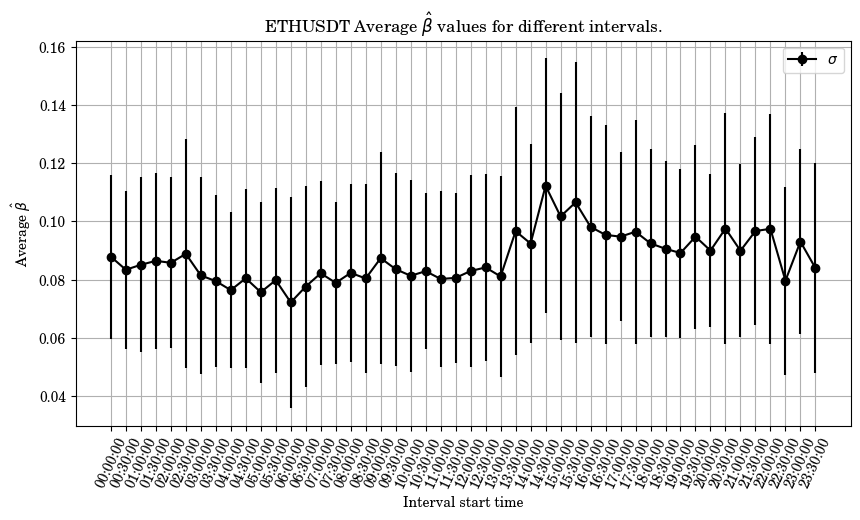
\includegraphics[width=0.8\textwidth]{./images/ETHUSDT_beta_across_time.png}
    \caption{ETHUSDT Average price impact coefficients for different half-hour intervals. Note that errorbars represent standard deviations.}
\end{figure*}

\begin{figure*}[htpb]
    \centering
    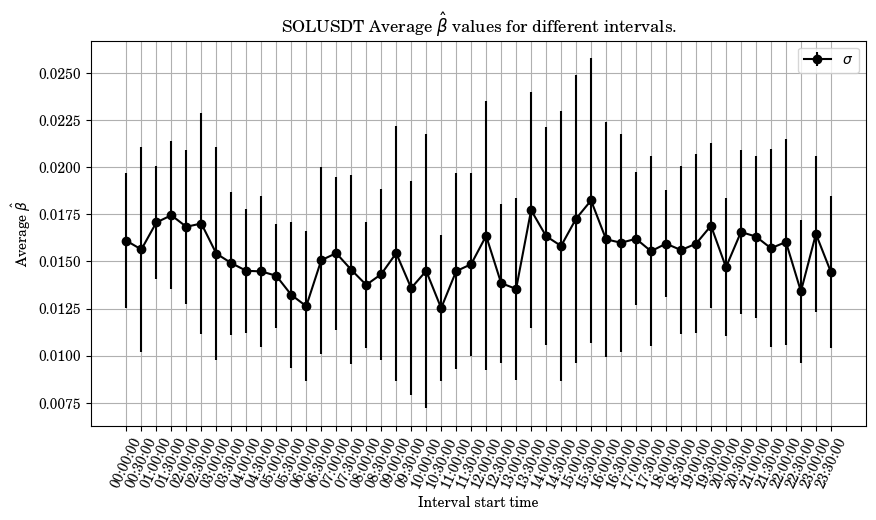
\includegraphics[width=0.8\textwidth]{./images/SOLUSDT_beta_across_time.png}
    \caption{SOLUSDT Average price impact coefficients for different half-hour intervals. Note that errorbars represent standard deviations.}
\end{figure*}

\begin{figure*}[htpb]
    \centering
    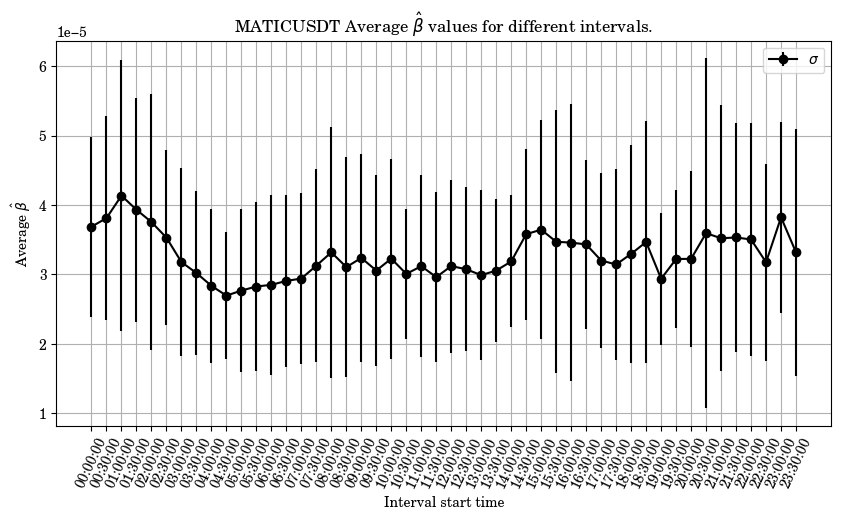
\includegraphics[width=0.8\textwidth]{./images/MATICUSDT_beta_across_time.png}
    \caption{MATICUSDT Average price impact coefficients for different half-hour intervals. Note that errorbars represent standard deviations.}
    \label{fig:MATICUSDT_beta_across_time}
\end{figure*}


% \subsubsection{From Contemporaneous to Predictive}
% Up until this point our regressions have all been contemporaneous, i.e
% we have been modelling a price change over some period using the sum of individual
% price changes over the same period. So one could argue that of course there is going
% to be a strong linear relationship. \cite{CONT2013} are more interested in 
% modelling the linear instantaneous price impact, rather than predicting future price movement.
%
% However in this paper we are also interested in future price movement prediction.
% To this end, we will now focus on predicting the labels as defined in (\ref{equation:modelling_objective}) for the remainder of this paper.
%
% Firstly we choose $\epsilon$ so that our decision rule is given by:
% \begin{equation}
%     \hat{y}_t = f(\text{OFI}(t)) := \text{sign}(\text{OFI}(t)) =  \begin{cases}
%         1 & \text{if } \text{OFI}(t) > 0\\
%         0 & \text{if } \text{OFI}(t) = 0 \\
%         -1 & \text{if } \text{OFI}(t) < 0
%     \end{cases}
% \end{equation}
%
% Since we have no hyperparameters and we are only using a simple decision rule, we can initially simply evaluate this model on the entire
% dataset without need for a separate validation set. We present these results  (with $h=1000ms$) in Table \ref{table:three_class}.
%
% \begin{table}[ht!]
% \resizebox{\textwidth}{!}{
% \begin{tabular}{lrllll}
% \hline
% Symbol & Accuracy & TP & Precision & Recall & F1 \\
% \hline
% BTCUSDT & 0.24 & (1542339, 25, 1525203) & (0.24, 0.83, 0.24) & (0.71, 0.0, 0.71) & (0.36, 0.0, 0.35) \\
% ETHUSDT & 0.24 & (1677501, 13, 1654539) & (0.25, 0.65, 0.24) & (0.69, 0.0, 0.69) & (0.36, 0.0, 0.36) \\
% SOLUSDT & 0.35 & (2308897, 23757, 2318412) & (0.35, 0.57, 0.35) & (0.62, 0.0, 0.62) & (0.44, 0.01, 0.45) \\
% MATICUSDT & 0.18 & (1041382, 12420, 1026689) & (0.18, 0.87, 0.18) & (0.66, 0.0, 0.65) & (0.29, 0.0, 0.29) \\
% \hline
% \end{tabular}
% }
% \caption{Initial three class classification results using a simple decision rule for $h=1000ms$.}
% \label{table:three_class}
% \end{table}
%
% So we see that we have pretty poor performance, with very low accuracies and poor precision
% for the -1 and +1 classes. Interestingly we observe decent performance for the +1 and -1 recalls,
% which means out of all the times when the true class is non-zero, our model does pretty well.
% To further examine this phenomena, we visually explore the distributions with more regression plots.
%
%
% \begin{figure}[htpb!]
%     \centering
%     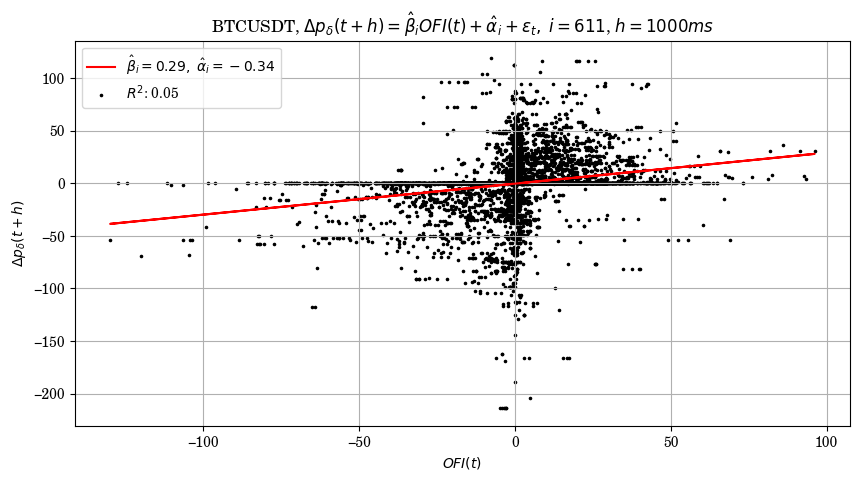
\includegraphics[width=1.0\textwidth]{./images/btcusdt_pred_OFI_three_class_h=1000ms.png}
%     \caption{OFI predictive regression for a given half-hour window for BTCUSDT.}
% \end{figure}
%
% \begin{figure}[htpb!]
%     \centering
%     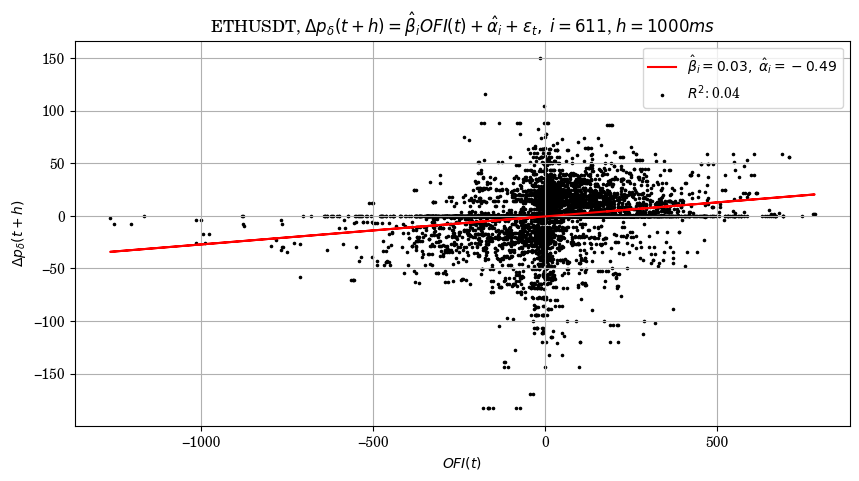
\includegraphics[width=1.0\textwidth]{./images/ethusdt_pred_OFI_three_class_h=1000ms.png}
%     \caption{OFI predictive regression for a given half-hour window for ETHUSDT.}
% \end{figure}
%
% \begin{figure}[htpb!]
%     \centering
%     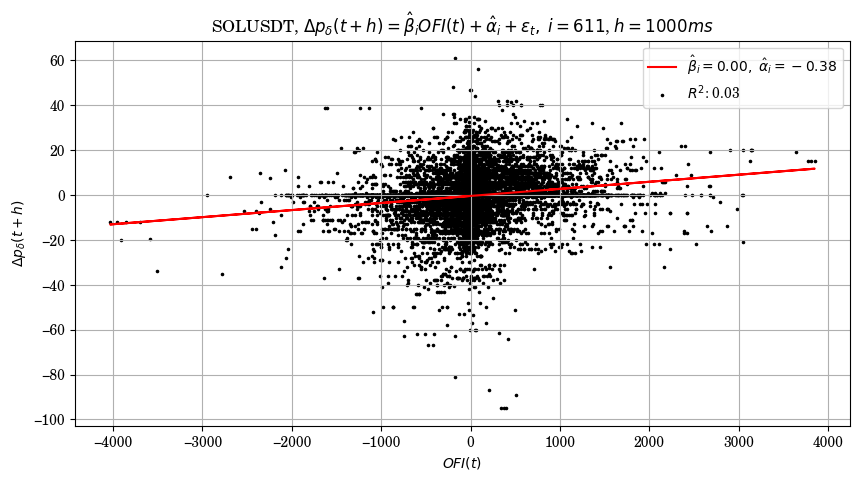
\includegraphics[width=1.0\textwidth]{./images/solusdt_pred_OFI_three_class_h=1000ms.png}
%     \caption{OFI predictive regression for a given half-hour window for SOLUSDT.}
% \end{figure}
%
% \begin{figure}[htpb!]
%     \centering
%     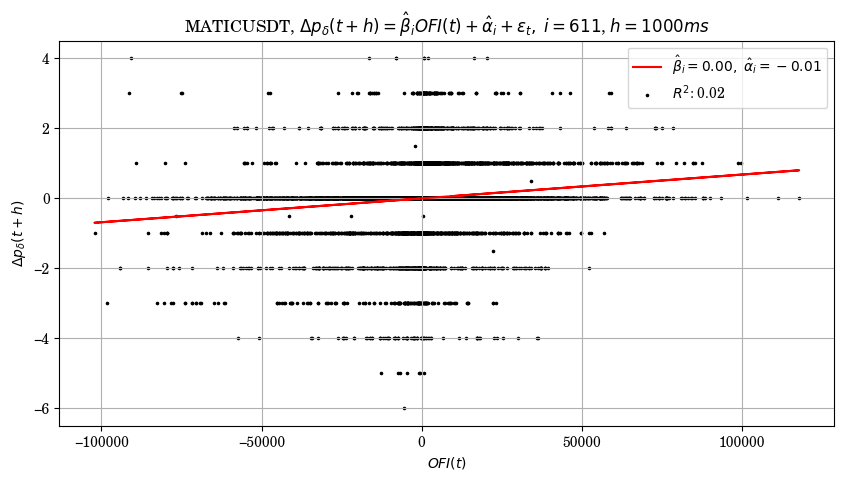
\includegraphics[width=1.0\textwidth]{./images/maticusdt_pred_OFI_three_class_h=1000ms.png}
%     \caption{OFI predictive regression for a given half-hour window for MATICUSDT.}
% \end{figure}
%
% Visually we see that OFI is a poor predictor of zero mid price change, however for non-zero
% price changes, there is a clear positive trend. To explore this further, we will remove
% all zero-price change observations from our data and we set $\epsilon = 0$,
% converting our multi-class classification into a binary classification problem.
% We define\footnote{Note that the choice of $\ge$ or $\le$ is inconsequential, since very few of our $\text{OFI}$ values
% are exactly zero.}
% our new decision rule, $f$ as:
%
% \begin{equation}
%     \hat{y}_t = f(\text{OFI}(t)) := \begin{cases}
%         1 & \text{if } \text{OFI}(t) \ge 0\\
%         -1 & \text{if } \text{OFI}(t) < 0
%     \end{cases}
%     \label{binary_decision_rule}
% \end{equation}
%
% We present the results of the modified classification (with $h=1000ms$) in Table \ref{table:binary_class}.
%
% \begin{table}[ht!]
% \resizebox{\textwidth}{!}{
% \begin{tabular}{lrllll}
% \hline
% Symbol & Accuracy & TP & Precision & Recall & F1 \\
% \hline
% BTCUSDT & 0.71 & (1542339, 1525204) & (0.71, 0.71) & (0.71, 0.71) & (0.71, 0.71) \\
% ETHUSDT & 0.69 & (1677501, 1654545) & (0.69, 0.69) & (0.69, 0.69) & (0.69, 0.69) \\
% SOLUSDT & 0.62 & (2308897, 2327249) & (0.62, 0.62) & (0.62, 0.62) & (0.62, 0.62) \\
% MATICUSDT & 0.66 & (1041382, 1027599) & (0.66, 0.66) & (0.66, 0.65) & (0.66, 0.65) \\
% \hline
% \end{tabular}
% }
% \caption{Classification results, when zero mid price change observations are excluded for $h=1000ms$.}
% \label{table:binary_class}
% \end{table}
%
% So we see that we have very good results when we exclude observations with no price change,
% which gives evidence to the idea that OFI is a good predictor of future non-zero price change.
%
% If we were to use this information to make informed trades, buying low and selling high and vice versa,
% then recall of the +1 and -1 classes would be most important,
% since missing a non-zero price change could be much more costly than falsely predicting a non-zero price change.
% For this simple application, if the actual price change is zero, we haven't lost any money.
%
% These results are for a horizon of $h=1000ms$. We now vary $h$ and report the accuracies in figure \ref{fig:OFI_accuracy_h}.
%
%  \begin{figure}[htpb]
%     \centering
%     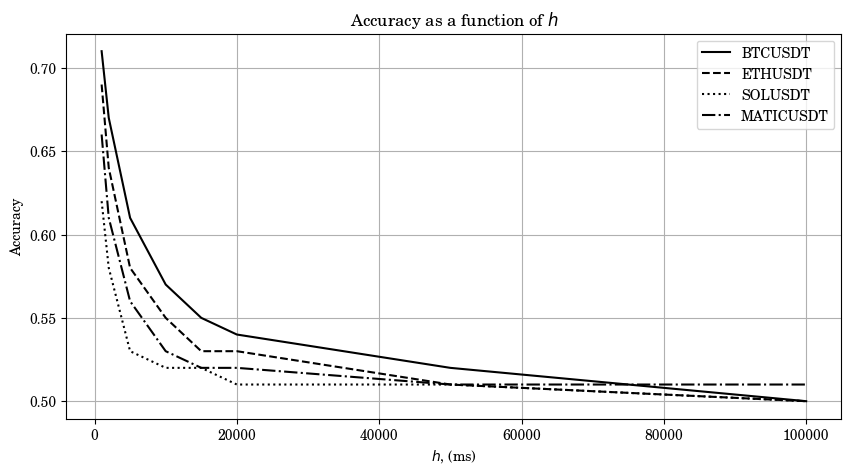
\includegraphics[width=1.0\textwidth]{./images/OFI_accuracy_h.png}
%     \caption{Prediction as a function of the prediction horizon, $h$. (With zero mid price change observations removed).}
%     \label{fig:OFI_accuracy_h}
% \end{figure}
%
% So we observe accuracy is decreasing in $h$, which is what we would expect, since longer
% horizons are in general harder to predict.
%
% We also see that for fixed $h$, BTCUSDT consistently has the highest accuracy, followed by ETHUSDT.
%
% Note that this $h$ is the lookback for $\text{OFI}(t)$ defined in (\ref{OFI})
% and also the lookahead for $y_t = f(\Delta p_{\delta}(t+h)) = f((p(t+h) - p(t)) / \delta)$.
% Until now we have used the same $h$ for both the lookahead and lookback. 
%
% We next explore how our model performs when we vary the lookahead and lookback independently.
% We denote our lookback to be $h_1$ and our lookahead to be $h_2$.
% So varying $h_1$ changes how far back we sum our $e_n$ values and varying $h_2$ changes
% how far into the future we are predicting the price change.
%
% We present our results in the below figures. Across all symbols we see that for a fixed lookahead, $h_2$, the accuracy
% is (mostly) decreasing in lookback, $h_1$. It seems that looking too far back into the past introduces noise
% and the price movements are not dependent on older order flow imbalances.
% We also see that for fixed lookbacks, $h_1$, the accuracy is decreasing in the lookahead, $h_2$.
% This is expected, as events further into the future are harder to predict.
%
% For all symbols we observe best accuracy with $h_1 = 1000ms$ and $h_2 = 1000ms$. So predicting
% short future horizons, with only recent information gives the best results.
%
% \begin{figure}[htpb!]
%     \centering
%     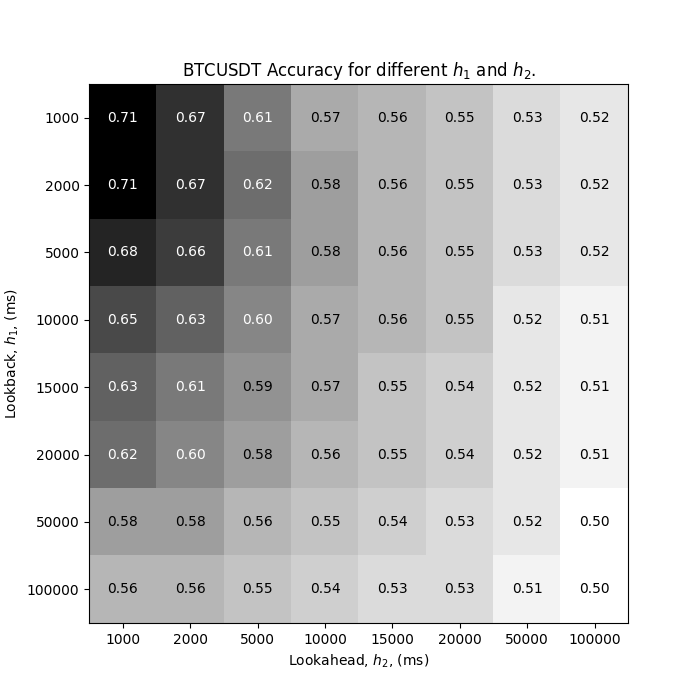
\includegraphics[width=0.7\textwidth]{./images/BTCUSDT_h1_h2_accuracy_heatmap.png}
%     \caption{Heatmap of accuracy when varying lookback, $h_1$ and lookahead, $h_2$ for BTCUSDT.}
% \end{figure}
%
% \begin{figure}[htpb!]
%     \centering
%     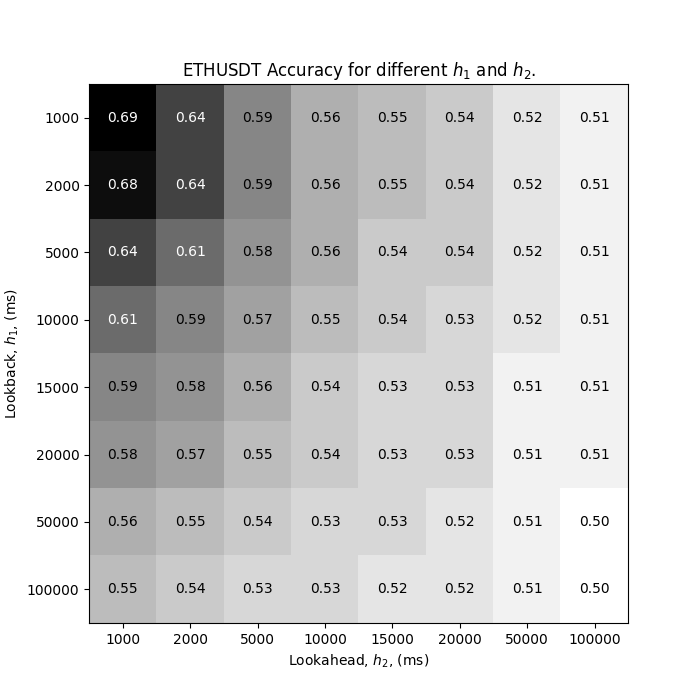
\includegraphics[width=0.7\textwidth]{./images/ETHUSDT_h1_h2_accuracy_heatmap.png}
%     \caption{Heatmap of accuracy when varying lookback, $h_1$ and lookahead, $h_2$ for ETHUSDT.}
% \end{figure}
%
% \begin{figure}[htpb!]
%     \centering
%     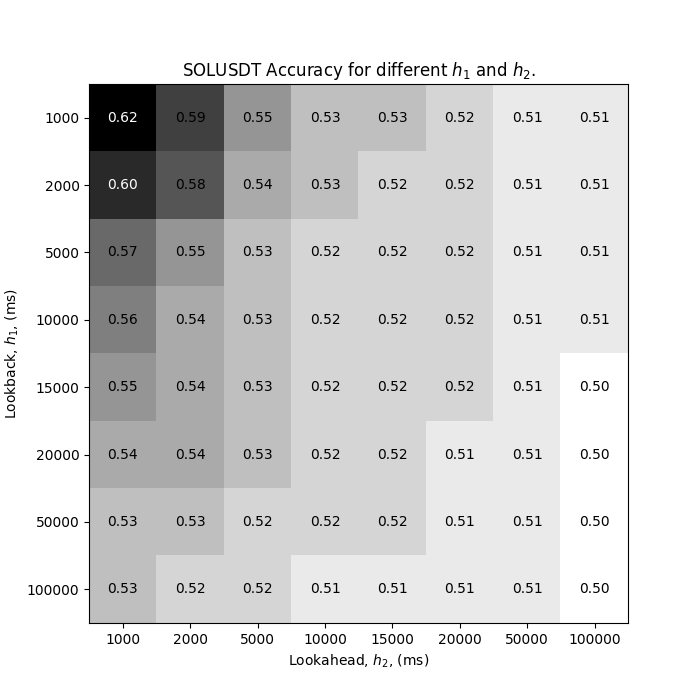
\includegraphics[width=0.7\textwidth]{./images/SOLUSDT_h1_h2_accuracy_heatmap.png}
%     \caption{Heatmap of accuracy when varying lookback, $h_1$ and lookahead, $h_2$ for SOLUSDT.}
% \end{figure}
%
% \begin{figure}[htpb!]
%     \centering
%     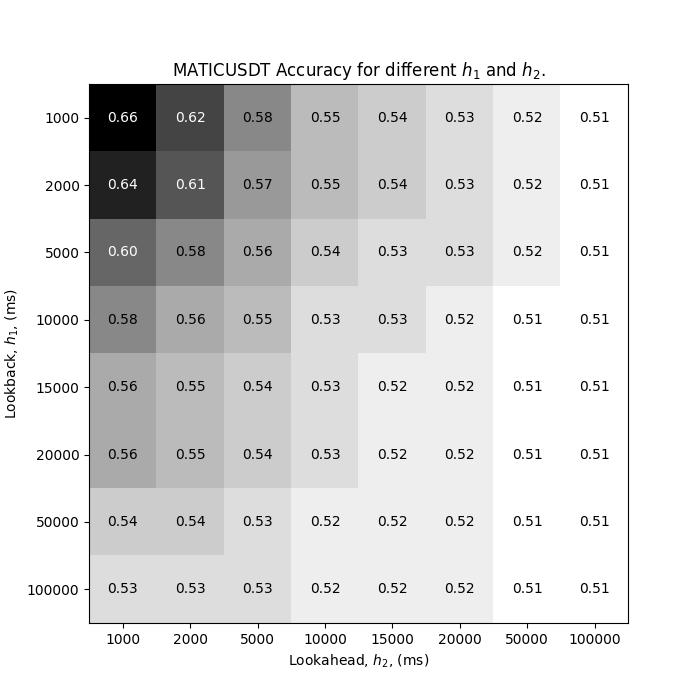
\includegraphics[width=0.7\textwidth]{./images/MATICUSDT_h1_h2_accuracy_heatmap.png}
%     \caption{Heatmap of accuracy when varying lookback, $h_1$ and lookahead, $h_2$ for MATICUSDT.}
% \end{figure}
%


\chapter{Predictive Modelling}
\section{The Modelling Objective}

Our main aim in this chapter is to predict future price movement.

Recall in (\ref{mid}) we defined the mid price, $p_0(t)$ to be the average of the best bid and ask prices at time $t$.

There are multiple possible modelling setups when it comes to mid price movement prediction.
\cite{KOLM2023} frame this as a regression problem, directly predicting future mid price values at multiple horizons.
\cite{ZHANG2019} and \cite{LUCCHESE2024} predict the sign of the returns, in a multi-class classification setting.
They argue that due to the highly stochastic nature of financial data, simply calculating labels based on returns from $p_{0}(t)$ and $p_{0}(t+k)$ 
leads to a label set with a lower signal to noise ratio, so smoothed returns are used.

In this paper we use the multi-class classification setup.
Following \cite{ZHANG2019}, we adopt the smoothed labelling method first introduced in \cite{AVRAAM2017}.

Define the quantites:
\begin{align}
    m_{-}(t) &:= \frac{1}{k} \sum_{i=0}^{k} p_0(t-i) \\
    m_{+}(t) &:= \frac{1}{k} \sum_{i=1}^{k} p_0(t+i) \\
    \ell(t) &:= \frac{m_{+}(t) - m_{-}(t)}{m_{-}(t)}
    \label{smoothed_returns}
\end{align}

So $m_{-}(t)$ represents the average price for the previous $k$ prices and current price
and $m_{+}(t)$ represents the average price for the next $k$ prices.
Then we calculate the smoothed returns $\ell(t)$ as the return of this smoothed price. 

Then we discretize these returns according to (\ref{desc}) in order to give us three distinct class labels for use in classification.

\begin{equation}
    y(t) = \begin{cases} \label{desc}
        +1  & \text{ if } \ell(t) \in (\epsilon, \infty) \\
        0  & \text{ if } \ell(t) \in [-\epsilon, \epsilon] \\
       -1  & \text{ if } \ell(t) \in  (-\infty, -\epsilon)
   \end{cases}
\end{equation}

So given the information we have up time $t$, our aim is to build a model that will
predict $y(t)$.

See Figure \ref{fig:example_mid_price_labelling} for a sample of our mid price data,
colour coded according to class label. We see regions of mid price downtrend are labelled
with -1 (coloured red), regions of mid price plateau are labelled with 0 (coloured blue)
and regions of mid price uptrend are labelled with +1 (coloured green).

\begin{figure*}[htpb]
    \centering \label{fig:example_mid_price_labelling}
    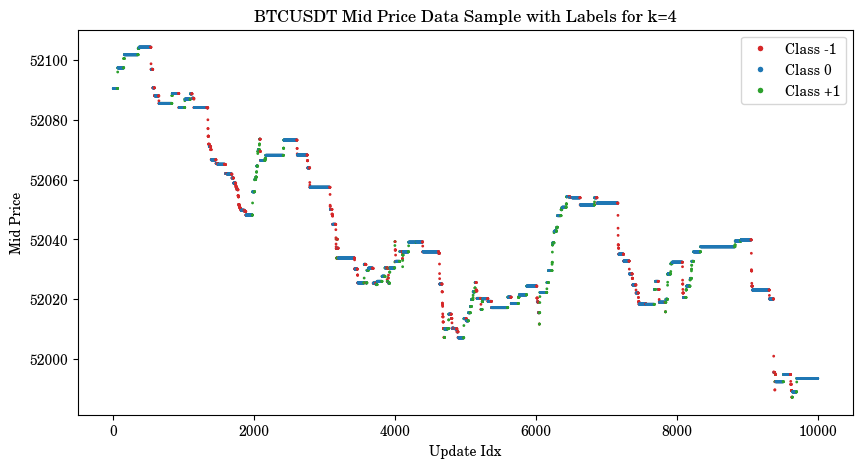
\includegraphics[width=1.0\textwidth]{./images/example_labels.png}
    \caption{An example BTCUSDT mid price sample, coloured according to class label.
    Note that the discretization parameter, $\epsilon$ is set $\approx 0$ and the prediction horizon is $k=4$ updates.}
\end{figure*}


Note that in some implementations, the prediction horizon is
given over some time interval, such as predicting the movement for the next 10 seconds.
In this paper, we instead define our prediction horizon in terms of ticks/updates/datapoints.
This choice was made, since our Websocket data arrives at irregular times, and for some short intervals
there is no available data. We expect the results to be very similar when using a time based horizon.


\section{Orderbook Features}
Now that we have our labels, we need to define our features.
We seek to define feature vectors $\bm{x}_t \in \mathbb{R}^d$ which capture the relevant orderbook 
information relating to future mid price movement. We can then learn a model of the form:
\begin{equation}
    \hat{y}(t) = \hat{f}(\bm{x}(t))
\end{equation}
that seeks to minimize some loss function w.r.t the true labels $y(t)$, i.e
\begin{equation}
   \hat{f} = \arg \min_{f} \mathcal{L}(\bm{y}, f(X))
\end{equation}

\subsection{Raw Orderbook Features}
\cite{ZHANG2019} use the raw orderbook data for their model input. I.e $\bm{x}(t)$ takes the form:
\begin{equation}
    \bm{x}(t) =: \bm{x}_t = [p_{t, \ell}^A, q_{t, \ell}^A, p_{t, \ell}^B, q_{t, \ell}^B]_{\ell=1}^{L} \in \mathbb{R}^{4L}
    \label{LOB_feature_vector}
\end{equation}
Where $L$ represents the maximum orderbook level in the data. For our data we have 10 orderbook
levels, so $L=10$. It is important to note that this is a non-stationary series.
It also combines price and volume information, which have different units, which is not ideal for most models.
From henceforth, we shall refer to this feature vector as the LOB (Limit OrderBook) feature vector.


\subsection{Orderflow Features}
\cite{KOLM2023} extend the idea of OFI, defined in (\ref{eBeA}), beyond the first level.
Define \footnote{We interchangeably use the notation $p_t := p(t)$.} the contribution of
the $n^\text{th}$ event at level $\ell$ on the (A)sk/(B)id side as: 
\begin{align}
    e_{t,\ell}^{A} &:=  I_{\{ p_{n, \ell}^A \leq p_{n-1,\ell}^A \}} q_{n}^A - I_{\{ p_{n, \ell}^A \geq p_{n-1, \ell}^A \}} q_{n-1, \ell}^A \\
    e_{t, \ell}^{B} &:= I_{\{ p_{n, \ell}^B \geq p_{n-1, \ell}^B \}} q_{n, \ell}^B - I_{\{ p_{n, \ell}^B \leq p_{n-1, \ell}^B \}} q_{n-1, \ell}^B
\end{align}
Then we define the Orderflow feature vector as:
\begin{equation}
    \bm{x}_t := [e_{t, \ell}^{A}, e_{t, \ell}^{B}]_{\ell=1}^L \in \mathbb{R}^{2L} \label{OF_feature_vector}
\end{equation}
This feature vector is stationary and is given in units of volume, so is consistent across dimensions.
It is also half the dimension of the LOB feature vector, a desirable property for the convergence of many models.

From henceforth, we shall refer to this feature vector as the OF (OrderFlow) feature vector.




\section{Model Architectures}

\subsection{Logistic Regression}
Linear regression is one of the oldest and most robust predictive models used in all areas
of science. It's simplicity, explainablity and robustness means it is a common choice for a baseline/benchmark
model.

Logistic regression, first introduced in \cite{COX1958}, is the natural extension of linear regression to the classification setting.

The key idea is to model the \textit{log odds} as linear functions of our data.

Suppose we have $C$ classes, indexed by $1, 2, \cdots, C$, then we assume the following linear model: 
\begin{align*}
    \log \frac{\mathbb{P}(Y=1 | X = x)}{\mathbb{P}(Y=C | X = x)} &= \alpha_1 + \beta_1' x \\
   \log \frac{\mathbb{P}(Y=2 | X = x)}{\mathbb{P}(Y=C | X = x)} &= \alpha_2 + \beta_2' x \\
   \vdots \\
   \log \frac{\mathbb{P}(Y=C-1 | X = x)}{\mathbb{P}(Y=C | X = x)} &= \alpha_{C-1} + \beta_{C-1}' x
\end{align*}

Note that because the probablities must sum to $1$, we have $C-1$ degrees of freedom.
Also note that the choice of denominator is not important as the model is equivariant
under the choice of denominator class.

With some re-arrangement, we get the posterior probabilities:
\begin{align*}
    \mathbb{P}(Y=c | X = x) &= \frac{\exp(\alpha_c + \beta_c' x)}{1 + \sum_{\ell=1}^{C-1} \exp(\alpha_{\ell} + \beta_{\ell}'x)} \\
    \mathbb{P}(Y=C | X = x) &= \frac{1}{1 + \sum_{\ell=1}^{C-1} \exp(\alpha_{\ell} + \beta_{\ell}'x)}
\end{align*}
Where  $c \in {1, 2, \cdots, C-1}.$

Interestingly we note that the log odds representation is equivalent to a bijective mapping of the linear functions $\alpha_c + \beta_c'x$ onto $[0, 1]$ using
the sigmoid function: $1 / 1 + \sigma(-x)$.

Note that the parameters $(\alpha_c, \beta_c)_{c=1}^C$ are fit by maximizing the log-likelihood using gradient descent methods.

So given some observation, $\bm{x}_t$, our model gives us the posterior probabilities of the observation
belonging to each class. In order to make a classification, we can simply choose the class with the highest
posterior probability, and assign this class to $\hat{y}_t$.

We refer the interested reader to \cite{HASTIE2001} for a more in depth exposition of the theory.

For our use case, we will define two logistic regression models, one using the LOB feature vectors first introduced in \ref{LOB_feature_vector}
and the other using the OF features introduced in \ref{OF_feature_vector}. 
From henceforth we will refer to these models as lrLOB and lrOF respectively.

Of course, when dealing with timeseries modelling, it is also important to incorporate autoregressive
features that allow the model to see previous observations for some lookback window.

We define our lookback window to be the previous $T$ observations. We incorporate these into
our model by concatenating lagged versions of the feature vector. I.e our model inputs will be:
\begin{equation}
    \bm{x}^{AR}_t = [\bm{x}_t; \bm{x}_{t-1}; \bm{x}_{t-2}; \cdots; \bm{x}_{T-1}] \in  \mathbb{R}^{dT}\label{AR_features}
\end{equation}

This will be the input to our logistic regression models.
The output will be $\hat{y}_t \in \{-1, 0, 1\}$

Note that we choose $T=10$, since larger values of $T$ will hurt the convergence
of the fitting algorithm and take too much memory and too long to fit.

This is a major limitation of this model and in later sections we introduce models
designed to handle much larger lookback windows.

\subsection{Decision Trees and XGBoost}
\textit{Decision Trees} are another very popular class of machine learning models with a
large amount of success in a wide range of fields. There are two main types; decision trees
for classification and decision trees for regression. The theory for both is very similar
and they share the same ideas. We focus on classification here.

The main idea is to learn an \textit{optimal} partition of our data using binary trees,
with each non-leaf node representing a split of our data on one variable.
The model learns which features to split on at each level and which threshold values to use for the splits.


More formally, following \cite{HASTIE2001}, suppose our data is $X \in  \mathbb{R}^{n \bm{x} d}$, then
we seek to partition our data into $M$ regions, $R_1, R_2, ..., R_M$, and then our prediction is given by:
\begin{equation}
    \hat{y}(x) = \sum_{m=1}^{M} c_m 1\{x \in  R_m\} 
\end{equation}

Where $c_m$ is the most common class in region $R_m$, i.e
\begin{equation}
    c_m = \arg \max_{c \{\in {1, 2, ..., C}\}} |\{y_i : y_i = c \land x_i \in R_m\}|
\end{equation}

Consider splitting our data with feature $j$, and threshold $s$. We denote the resulting
partitions with $R_1$ and $R_2$, defined as: 
\begin{equation}
    \begin{aligned}
        R_1(j, s) &:= \{X : X_j \le s\}, \\
        R_2(j, s) &:= \{X : X_j >  s\} 
    \end{aligned}
\end{equation}

The \textit{optimal} $j$ and $s$ are chosen to solve:
\begin{equation}
    j^*, s^* = \arg \min_{j,s}  \mathcal{L}(R_1(j, s), R_2(j, s))
\end{equation}
Where $\mathcal{L}$ is some loss function measuring how well the partition splits the data.

Since checking all combinations of features and threshold values would be computationally infeasible, the fitting
algorithm uses an iterative greedy approach, choosing the optimal splits at each level based on some loss function that
measures how well the split partitions the data for the next level.

One commonly used loss function is the misclassification error:
\begin{equation}
    \begin{aligned}
        \mathcal{L}(R_1, R_2) &= \min_{c_1} \frac{1}{n_1} \sum_{x_i \in  R_1(j, s)} 1(y_i \neq c_1) \\
                    &+ \min_{c_2}\frac{1}{n_2} \sum_{x_i \in  R_2(j, s)} 1(y_i \neq c_2)
    \end{aligned}
\end{equation}

In practice it has been found that other loss functions, such as \textit{cross-entropy} or \textit{gini impurity} give better results.
They are also differentiable which is better for certain optimization algorithms. We again refer the interested reader to \cite{HASTIE2001}
for a more in depth discussion of these details.

Simple decision trees have high variance, meaning they can easily overfit to training data.
For this reason, various \textit{ensemble} methods were devised to reduce overfitting.

We introduce one such method, \textit{Boosting}. The basic idea is to iteratively train many \textit{weak learners}
and then combine their predictions to produce a single, more robust prediction. Weak learners are simple models
which are only slightly better than randomly guessing and 
have low variance and high bias. In theory, by combining many weak learners, 
boosting lowers the model bias, whilst keeping variance low.

In more detail, in each iteration, we fit a weak classifier (e.g a single decision tree stump),
We then compute the error according to some loss function. Then we use this error to define the weight for the current iteration,
then we re-weight our training data, using this weight, so samples where the model performed badly are given more weight in the next iteration.
Then our final output model will be a weighted sum of the predictions of the weak learners.

See figure \ref{fig:weaklearner} for a visualization of an example weak learner.

XGBoost, first introduced in \cite{XGBOOST2016}, is an extremely efficient implementation of Boosted Decision Trees.
We choose XGBoost as one of our models for several reasons.
Firstly XGBoost has been shown to be highly effective in a wide range of applications.
It has great representational capacity, with the ability to capture high dimensional, non-linear relationships
in the data, with tight control of overfitting.
It handles high dimensional data well, with feature sub-sampling helping to reduce overfitting.
It also has great explainability, with the ability to rank features by importance (which we will explore in a later section).
As an added bonus, it can be run on a GPU, allowing for very fast training and inference.
Interestingly there is little to no mention of its use for limit orderbook prediction in the literature,
and we believe it has great potential for this purpose.

XGBoost has many hyper-parameters that one can tune. We finetune our models on the validation windows and 
present our finetuned hyperparameters along with their definitions here:
 \begin{itemize}
    \item \textbf{max depth} = 3. The max depth of each weak learner tree.
    \item \textbf{eta} = 0.1. Similar to learning rate, influences weighting.
    \item \textbf{data subsample ratio} = 0.8. The proportion of the training data that each weak learner can use.
    \item \textbf{column subsample ratio} = 0.8. The proportion of the features available when performing splits.
    \item \textbf{evaluation metric} = Multiclass classification error rate. The metric used during the boosting algorithm to determine weights.
\end{itemize}


Similar to our logistic regression models, we define two XGBoost models, one using the LOB feature vectors first introduced in \ref{LOB_feature_vector}
and the other using the OF features introduced in \ref{OF_feature_vector}. 
From henceforth we will refer to these models as xgbLOB and xgbOF respectively.

As before, we use the autoregressive feature concatenation introduced in \ref{AR_features}, with the same lookback, $T = 10$.

\begin{figure}[htpb]
    \centering
    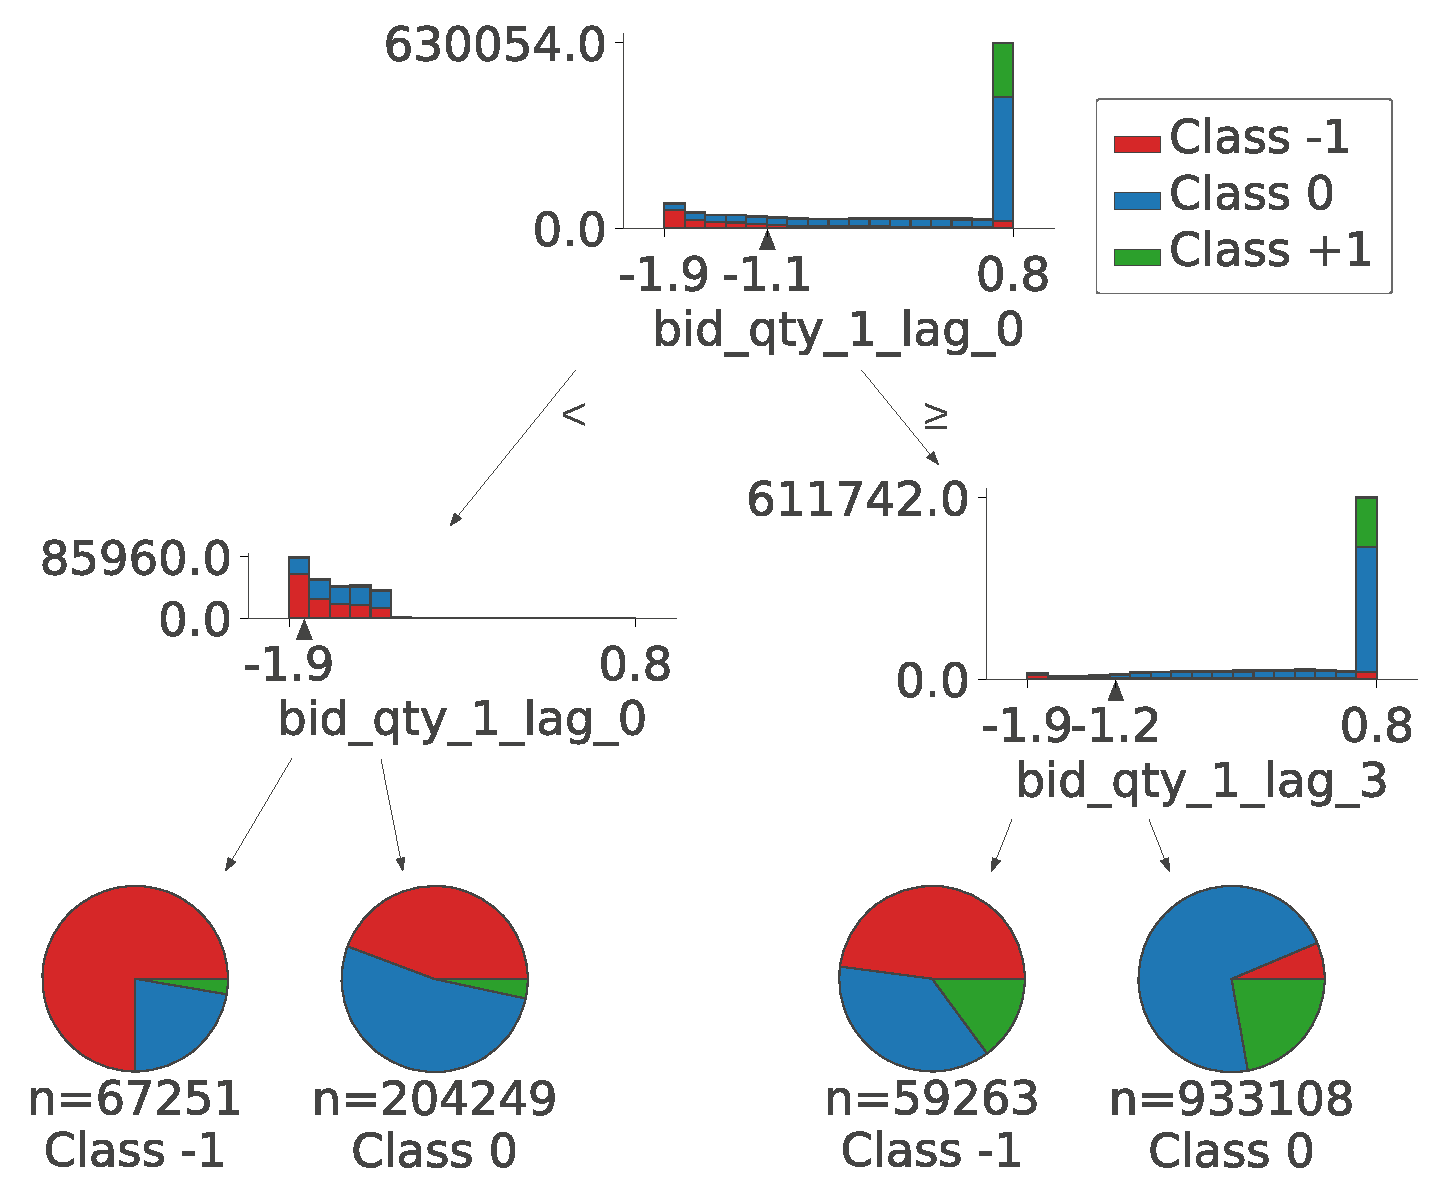
\includegraphics[width=0.8\textwidth]{./images/xgb_viz.pdf}
    \caption{A visualization of a single XGBoost weak learner with max depth set to 2.}
    \label{fig:weaklearner}
\end{figure}


\subsection{Artificial Neural Networks}
Artificial Neural Networks are a broad class of machine learning model that can efficiently approximate
high dimensional non-linear functions. Perhaps the most famous and example of an ANN (Artifical Neural Network)
is that of the Multi-layer Perceptron, first introduced in \cite{ROSENBLATT1958}. The basic idea is to take some input
vector and successively project it onto new spaces with affine and then non-linear transformations.

An MLP with $N$ hidden layers can be defined mathematically as:
\begin{equation}
    \begin{aligned}
        f_i(x; W_i, b_i) &= \sigma_i(W_i x + b_i) \\
        f(x; W_1, W_2, ..., W_N, b_1, b_2, ..., b_N) &= f_N \circ f_{N-1} \circ ... \circ f_2 \circ f_1(x)
    \end{aligned}
\end{equation}
Where $W_i$  are learnable weight matrices, $b_i$ are learnable bias vectors, $\sigma_i$ are fixed non-linear activation functions and $\circ$ denotes function composition.

MLPs are powerful because, as \cite{HORNIK1989} shows, they are \textit{universal function approximators}.
This means that, with as few as one hidden layer and using arbitrary activation functions, 
they are capable of approximating any Borel measurable function from one finite dimensional space 
to another to any desired degree of accuracy, provided sufficiently many hidden units are available.

The weight matrices and bias vectors are learnt by minimizing some loss function.
If we denote our learnable parameters as $\theta$, then our loss function is given by:
\begin{equation}
   \mathcal{L} (\theta; x, y) := \frac{1}{n} \sum_{i=1}^{n} \ell(f(x_i; \theta), y_i)
\end{equation}
Where $\ell$ is some observation-wise loss that measures how well our model predicts
$y_i$ given corresponding input $x_i$.

For simple problems $\mathcal{L}$ is commonly a convex function and so gradient descent methods can be
used to perform the minimization. E.g for vanilla gradient descent, one might define the update rule as:

\begin{equation}
    \theta^{(t+1)} \gets \theta^{(t)} - \eta \nabla_\theta \mathcal{L}(\theta^{(t)})
\end{equation}

In practice the optimization problem is often not convex, with many local minima, and so alternative optimization methods
are often used, such as \textit{Stochastic Gradient Descent} \cite{ROBBINS1951} or \textit{ADAM} \cite{ADAM2017}.

Stochastic Gradient Descent is a stochastic approximation of the gradient descent method, that
evaluates the gradient on a randomly sampled subset of the training data, instead of the entire training data.
It can be shown \textbf{TODO: CITATION} that the stochastic approximation of the gradient converges in expectation to
the gradient evaluated on the entire training dataset.

This sub-sampling allows for fewer gradient evaluations and therefore faster training. Also the stochastic
nature of the algorithm means it is less likely to get stuck in local minima.

ADAM, first introduced in \cite{ADAM2017}, is more advanced type of Stochastic Gradient Descent
that uses the concept of \textit{Momentum}, \cite{RUMELHART1986}. Momentum accumulates
the gradient from past updates to help guide the direction of the current step. It helps
to reduce oscillations during descent and often leads to faster convergence.

The ADAM update step is given by:
\begin{equation}
    \begin{aligned}
        m_{\theta}^{(t+1)} &\leftarrow \beta _{1}m_{\theta}^{(t)}+\left(1-\beta _{1}\right)\nabla_{\theta} \mathcal{L}(\theta^{(t)}) \\
        v_{\theta}^{(t+1)} &\leftarrow \beta _{2}v_{\theta}^{(t)}+\left(1-\beta _{2}\right)\left(\nabla_{\theta} \mathcal{L}(\theta^{(t)})\right)^{2} \\
        {\hat {m}}_{\theta} &={\frac {m_{\theta}^{(t+1)}}{1-\beta _{1}^{t}}} \\
        {\hat {v}}_{\theta} &={\frac {v_{\theta}^{(t+1)}}{1-\beta _{2}^{t}}} \\
        \theta^{(t+1)} &\leftarrow \theta^{(t)}-\eta {\frac {{\hat {m}}_{\theta}}{{\sqrt {{\hat {v}}_{\theta}}}+\delta }}
    \end{aligned}
\end{equation}
So we see that ADAM uses exponential moving averages with decay factors $\beta_1$ and $\beta_2$ to accumulate first and
second gradient moments. Note that $\delta$ is some small constant, used to prevent zero division errors.

Using traditional differentiation methods, the $\nabla_\theta \mathcal{L}(\theta^{(t)})$ calculation would be very computationally
expensive and training would be too slow to be practical. Instead, an algorithm called \textit{backpropagation}, \cite{RUMELHART1986},
can be used to efficiently differentiate the network with respects to the weights and biases. 
Backpropagation is an efficient implementation of the chain rule for differentiation that uses
dynamic programming to avoid repeated calculations. The idea is to construct a \textit{computational} graph,
which is a graph datastructure, where nodes represent functions and the edges represent function compositions.
So by doing a \textit{forward pass} of the graph, we are essentially evaluating the network given some input.
We then get an output, and do a \textit{backward pass} to accumulate gradients in an efficient way using the chain rule.
Backpropagation has computational complexity of the order of the number of edges in the computational graph,
so for large networks it scales very well and can be made to run extremely efficiently.

\subsection{Convolutional Neural Networks}

Convolutional Neural Networks (CNNs) are a specialized class of artificial neural 
networks designed primarily for processing structured grid data, such as images.

First introduced in \cite{LECUN1998}, CNNs have become a cornerstone in the field of
computer vision due to their ability to efficiently capture spatial hierarchies in data.

The fundamental building block of a CNN is the convolutional layer, which applies a
series of learnable filters (or kernels) to the input data.
Each filter \textit{convolves} across the input.
Mathematically, the output of a convolutional layer can be expressed as:
\begin{equation}
    h_{ij} = \sigma\left((W * x)_{ij} + b\right)
\end{equation}
where $W$ are the learnable filters, $b$ are the learnable biases,
$*$ denotes the convolution operation, and $\sigma$ is a non-linear 
activation function applied element-wise.

Note that for a $k\times k$ filter, the discrete convolution operation is defined as:
\begin{equation}
    (W * x)_{ij} := \sum_{m=-k}^{k}\sum_{n=-k}^{k} W_{mn} x_{i-m, j-n}
\end{equation}

So essentially we're sliding a window/filter over our 2D data and taking the dot product
at each position, resulting in a new 2D output for each filter.
This means the number of 2D outputs (\textit{channels}) is equal to the number of filters
for that layer.

The convolutional operation is a vector product and is differentiable with respect to
the filters, so we can simply apply gradient descent, just the same as with ANNs,
to learn our filters and biases.

In addition to convolutional layers, we also introduce \textit{pooling layers} 
which down-sample the spatial dimensions of the input, reducing computational
complexity and aiding in hierarchical feature extraction. 
The most common type of pooling is max-pooling, defined as:
\begin{equation}
    h_{ij} = \max_{(m,n) \in P_{ij}} x_{mn}
\end{equation}
where \(P_{ij}\) represents a pooling region around position $(i,j)$.


CNNs are powerful because they leverage three important ideas: local receptive fields, 
shared weights, and spatial subsampling. These ideas enable CNNs to only look at relevant information,
be much more computationally efficient and also to be invariant to small translations, scale, and distortions.
\textbf{TODO: Add more citations}

\subsection{Long Short Term Memory}

First introduced in \cite{HOCHREITER1997}, A (L)ong (S)hort-(T)erm (M)emory 
is a special type of (R)ecurrent (N)eural (N)etwork.
RNNs are neural networks that take in sequences of input iteratively. At each iteration,
they take in the previous \textit{hidden state} and the current input and then update
the hidden state and give an output. This hidden state mechanism allows them 
to \textit{remember} long term dependencies between inputs and they are often used to learn temporal dependencies in timeseries data.
One of the most famous simple RNNs is the Jordan network, introduced in \cite{JORDAN1997},
where the hidden state at each iteration, $h_t$ and the output $y_t$ are given by:
\begin{equation}
    \begin{aligned}
        h_t &= \sigma_h(W_h x_t + U_h y_{t-1} + b_h)  \\
        y_t &= \sigma_y(W_y h_t + b_y)
    \end{aligned}
\end{equation}
Where $x_t, h_t, y_t$ are the input, hidden state and output at iteration $t$ respectively.
$W, U$ and $b$ are all learnable parameter matrices/vectors and $\sigma_h$ and $\sigma_y$ are activation functions.

Whilst in theory, simple RNNs should be able to remember any length dependency, in practice
they suffer from the \textit{vanishing gradients problem} \cite{PASCANU2013}, where
gradients converge to zero during training, and therefore learning stops.

LSTMs were designed to address this problem, with special \textit{forget gates} which
learn to forget irrelevant information.

The most common type of LSTMs are composed of an \textit{input gate}, \textit{output gate}, \textit{forget gate}
and a \textit{cell}. The cell learns the information and the other gates regulate the flow of information from/to the cell.

Mathematically this looks like:
\begin{equation}
    \begin{aligned}
        f_t &= \sigma_g(W_f x_t + U_f h_{t-1} + b_f) \\
        i_t &= \sigma_g(W_i x_t + U_i h_{t-1} + b_i) \\
        o_t &= \sigma_g(W_o x_t + U_o h_{t-1} + b_o) \\
        \tilde{c}_t &= \sigma_c(W_c x_t + U_c h_{t-1} + b_c) \\
                c_t &= f_t \odot c_{t-1} + i_t \odot \tilde{c}_t \\
        h_t &= o_t \odot \sigma_h(c_t)
    \end{aligned}
\end{equation}

Where $\odot$ denotes the element-wise product. \cite{SCHMIDHUBER1999}
So essentially we are just expanding on the idea of the RNN with more hidden state
for greater control over what information is learnt.

Just like any other neural network, RNNs and LSTMs can be trained by gradient descent
with backpropagation.

\clearpage

\subsection{DeepLOB}
First introduced in \cite{ZHANG2019}, the DeepLOB model is a deep neural network
that uses a combination of convolutional and LSTM layers to extract short and long term
features from the raw orderbook data.

In this section we give a general overview of this model, but we refer the interested
reader to \cite{ZHANG2019} for a more in depth exposition.

Firstly, it is important to understand the structure of the model input in order
to understand the convolutional filter dimension choices.
The model input is a vertical concatenation of our LOB feature
vectors, denoted by $X_t \in \mathbb{R}^{T \times 4L}$, where $X_t :=$
\begin{equation*}
\begingroup
\setlength\arraycolsep{1pt}
\begin{bmatrix}
p_{t-T, 1}^A & q_{t-T, 1}^A & p_{t-T, 1}^B &  q_{t-T, 1}^B &  \cdots & p_{t-T, L}^A &  q_{t-T, L}^A & p_{t-T, L}^B & q_{t-T, L}^B\\
p_{t-(T-1), 1}^A & q_{t-(T-1), 1}^A & p_{t-(T-1), 1}^B &  q_{t-(T-1), 1}^B &  \cdots & p_{t-(T-1), L}^A &  q_{t-(T-1), L}^A & p_{t-(T-1), L}^B & q_{t-(T-1), L}^B\\
\vdots & \vdots & \vdots & \vdots & \ddots & \vdots & \vdots& \vdots & \vdots\\
p_{t-1, 1}^A & q_{t-1, 1}^A & p_{t-1, 1}^B &  q_{t-1, 1}^B &  \cdots & p_{t-1, L}^A &  q_{t-1, L}^A & p_{t-1, L}^B & q_{t-1, L}^B\\
p_{t, 1}^A & q_{t, 1}^A & p_{t, 1}^B &  q_{t, 1}^B &  \cdots & p_{t, L}^A &  q_{t, L}^A & p_{t, L}^B & q_{t, L}^B\\
\end{bmatrix}
\endgroup
\end{equation*}
(Note that if we reshape and flatten this matrix, we recover our autoregressive LOB feature vector defined in (\ref{AR_features}),
however in this case, we can use a much larger lookback without running out of memory, so we set $T=100$).

The DeepLOB model is comprised of three main modules, a convolutional module, an inception module and
an LSTM module. The output is then fed into a final linear layer before being passed through a softmax
function to give probabilities of each class, where the function $\text{softmax}: \mathbb{R}^d \to \Delta^{d-1}$
is defined element-wise as:
\begin{equation}
   \text{softmax}(x)_i = \frac{\exp(x_i)}{\sum_{j=1}^{d} \exp(x_j)}
\end{equation}

$\text{LeakyReLU}(x) := \max(0, x) + 0.01 * \min(0, x)$ \cite{MAAS2013} activation functions are used between each layer to introduce non-linearity.
Batch normalization is also used to ensure stable training.

We present a schematic of the DeepLOB model in Figure \ref{fig:DeepLOB} and dive deeper
into the architecture of the three main modules below.

\clearpage

\begin{multicols}{2}
\textbf{Convolutional Module:}
Conv 1 aggregates price and volume information for each level for each side,
Conv 2 aggregates information across side for each level and then
Conv 3 aggregates information across the whole orderbook.

The convolutional blocks use horizontal filters of dimension $1 \times 2$ with stride $1 \times 2$, in order
to combine price and volume information. Then they use vertical $4 \times 1$ convolutional filters to combine
information across time, $4$ timesteps at a time. Then the final convolutional block uses a $1 \times 10$ convolutional
filter to combine information across all 10 levels of the orderbook.

\textbf{Inception Module:}
The inception module has three blocks. The $1 \times 1$ filters increase the dimensionality of
the input and then the $3 \times 1$ and $5 \times 1$ simulate moving averages.
The main idea is to simulate a \textit{Network-In-Network}, \cite{MIN2014}.
A Network-In-Network essentially replaces the convolution operation with a small MLP
that is shared among all convolutional windows. The output is obtained by sliding the MLP
over the input in a similar manner as CNN.
The outputs of each inception block are then concatenated and reshaped into a $\mathbb{R}^{T \times 192}$ timeseries
which is then fed into the LSTM module.

\textbf{LSTM Module:}
The LSTM module is comprised of an LSTM layer with 64 hidden units. The purpose
of this layer is to capture long term dependencies from the inception output.

\columnbreak
\begin{figure}[H]
    \centering
    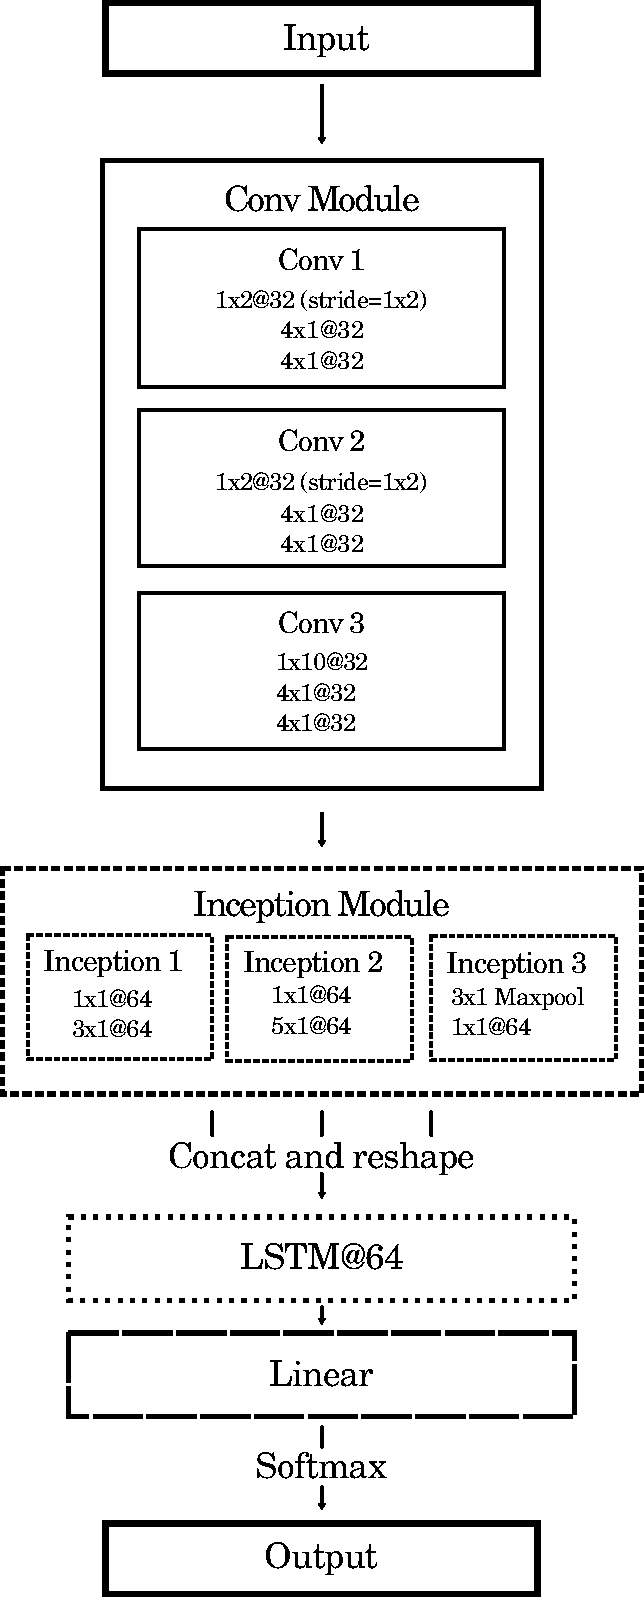
\includegraphics[width=0.45\textwidth]{./images/deepLOB_architecture_long.pdf}
    \caption{DeepLOB model architecture overview. Note: 1x2@32 denotes a convolutional layer with 32 filters and kernel size 1x2.}
    \label{fig:DeepLOB}
\end{figure}
\end{multicols}

\subsection{DeepOF}
Introduced in \cite{KOLM2023}, DeepOF is a modification of the DeepLOB architecture, to use
OF features, rather than LOB features. \cite{KOLM2023} show that using orderflow
instead of the raw orderbook representation leads to better performance.

The DeepOF input is given by:

\begin{equation}
X_{t} := \begin{bmatrix}
e_{t-T, 1}^A & e_{t-T, 1}^B &   \cdots & e_{t-T, L}^A & e_{t-T, L}^B \\
e_{t-(T-1), 1}^A & e_{t-(T-1), 1}^B &   \cdots & e_{t-(T-1), L}^A & e_{t-(T-1), L}^B \\
\vdots & \vdots & \ddots & \vdots & \vdots \\
e_{t-1, 1}^A & e_{t-1, 1}^B &  \cdots & e_{t-1, L}^A & e_{t-1, L}^B \\
e_{t, 1}^A & e_{t, 1}^B &  \cdots & e_{t, L}^A & e_{t, L}^B \\
\end{bmatrix} \in \mathbb{R}^{T \times 2L}
\label{DeepLOB_input}
\end{equation}
where we have extended the tick level orderflow definition from (\ref{eBeA}) to any arbitrary orderbook level, $\ell$:
\begin{equation}
    \begin{aligned}
        e_{t, \ell}^B &:= I_{\{p_{t, \ell}^B \ge p_{t-1, \ell}^B\}} q_{t, \ell}^B - I_{\{p_{t, \ell}^B \le p_{t-1, \ell}^B\}} q_{t-1, \ell}^B \\
        e_{t, \ell}^A &:= I_{\{p_{t, \ell}^A \le p_{t-1, \ell}^A\}} q_{t, \ell}^A - I_{\{p_{t, \ell}^A \ge p_{t-1, \ell}^A\}} q_{t-1, \ell}^A
    \end{aligned}
\end{equation}
In terms of model architecture, the DeepOF model is the same as the DeepLOB model, except without
the first convolutional block, Conv 1. Recall that this block aggregates the price and volume information
from the LOB input, so by using OF input, we have essentially aggregated the price and volume information manually
using a predefined feature transform that has been shown to be predictive of mid price movement. \cite{CONT2013}, \cite{KOLM2023}.

\section{Methodology}

\subsection{Sliding Window Setup}
We use a sliding window evaluation method, with train, validation and testing splits.
See figure \ref{fig:slidingwindow} for a visual representation
of the splits.

\begin{figure*}[htpb]
    \centering
    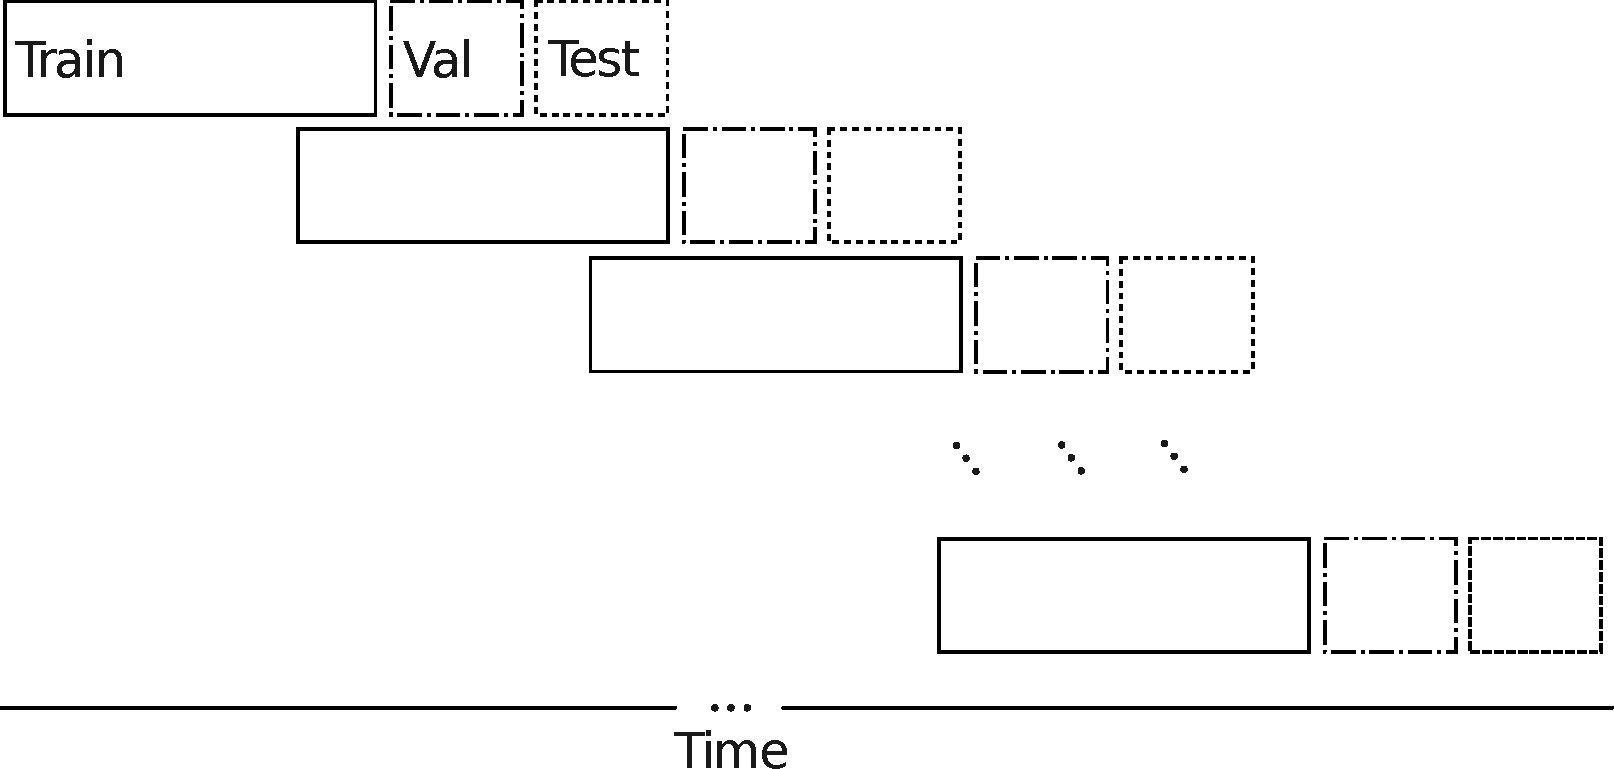
\includegraphics[width=1.0\textwidth]{./images/sliding_window.pdf}
    \caption{Sliding window visualization.}
    \label{fig:slidingwindow}
\end{figure*}

So using this method we are able to validate and test on almost the entire dataset,
and only train on recent, relevant information. Note that we leave gaps between the train,
val and test blocks to avoid data leakage from features that look back in time.

We fix the length of the initial training window to 48 hours and the validation and testing windows to 24 hours each.

The general testing procedure will be to train on the training set, then finetune our hyper-parameters using
the validation set, then once all of our hyper-parameters have been chosen, 
we will test on the test set. Of course this means there will be a gap of 24 hours between our training
and testing data. We could alternatively merge the training and validation data once hyperparameter tuning is
complete and then re-train our models on the merged data before testing. However, leaving this gap
will provide an extra guarantee of robustness and provide a better picture of the out of sample
performance of our models.

\subsection{Data Normalization}
For several of our models, data normalization is important in order to ensure stable training
and convergence. \cite{LUCCHESE2024} and \cite{ZHANG2019} use five day rolling window normalization
whereas \cite{KOLM2023} use $z$-scores calculated using the training data.
We find the rolling window normalization method to give worse performance, since it transforms
our data in a non-linear way and so, for example, periods of no price change are
no longer flat. So following \cite{KOLM2023}, for each train-val-test window we calculate the 
sample mean and standard deviation of the training data, and use this to scale the training,
validation and testing data, i.e 
\begin{equation}
    \begin{aligned}
        \hat{\mu}_{\text{train}} &:= \frac{1}{n_{\text{train}}} \sum_{i=1}^{n_{\text{train}}} X[i, :] \\
        \hat{\sigma}_{\text{train}} &:= \frac{1}{n_{\text{train}}} \sum_{i=1}^{n_{\text{train}}} (X[i, :] - \hat{\mu}_{\text{train}})^2 \\
        \tilde{X}_{\text{train}} &:= \frac{X_{\text{train}} - \hat{\mu}_{\text{train}}}{\hat{\sigma}_{\text{train}}} \\
        \tilde{X}_{\text{val}} &:= \frac{X_{\text{val}} - \hat{\mu}_{\text{train}}}{\hat{\sigma}_{\text{train}}} \\
        \tilde{X}_{\text{test}} &:= \frac{X_{\text{test}} - \hat{\mu}_{\text{train}}}{\hat{\sigma}_{\text{train}}}
    \end{aligned}
\end{equation}

\subsection{Choice of label discretization parameter}
Following \cite{LUCCHESE2024}, we set our discretization parameter, $\epsilon$, from (\ref{desc})
for each $k$ and train-val-test window, $w$, so that the classes are roughly balanced. I.e
\begin{equation}
    \epsilon := \epsilon_{k, w} := \frac{|\hat{F}_{k, w}^{-1}(\frac{1}{3})| + \hat{F}_{k, w}^{-1}(\frac{2}{3})}{2}
\end{equation}
Where $\hat{F}_{k, w}$ is the empirical distribution of the training set $\ell(t)$ (\ref{smoothed_returns}) smoothed returns 
for prediction horizon $k$, and window $w$.


\subsection{Model Training}
Our DeepLOB and DeepOF models were trained with PyTorch, \cite{PYTORCH2017},
on an Nvidia RTX 3060 12GB with 64GB memory and a 14-core 20-thread Intel i5 13600K.

We use the ADAM optimizer with learning rate set to $0.0001$.

For our loss function we use the Cross Entropy Loss, \cite{CROSSENTROPYLOSS},
which is basically a weighted $\log-\text{softmax}$.
% Our model 
% input is $(minibatch, C)$
% $$
% l_{n} = -w_{y_{n}} \log \frac{\exp(x_{n, y_{n}})}{\sum_{c=1}^C \exp(x_{n, c})}
% $$
% $$
% l(x, y) = \sum_{n=1}^N \frac{1}{\sum_{m=1}^N w_{y_{m}}} l_{n}
% $$
% ...

\section{Results}

\subsection{Model Results}


\subsection{Feature Importances}
Another advantage of using a decision tree based model is that we get easily explainable
feature importances. During training, we split the tree at each level, using the feature
that gives us the best partition according to some metric. We can use this fact
to rank features based on the number of times a feature was used to split the tree. We
denote this count as the \textit{weight} of the feature.
More influential features will have a higher weight since they are the best discriminators
of the data.

We plot the top 10 LOB features for xgbLOB BTCUSDT in figure \ref{top_10_lob_features} for different $k$, prediction horizons.
\begin{figure}[htpb]
    \centering
    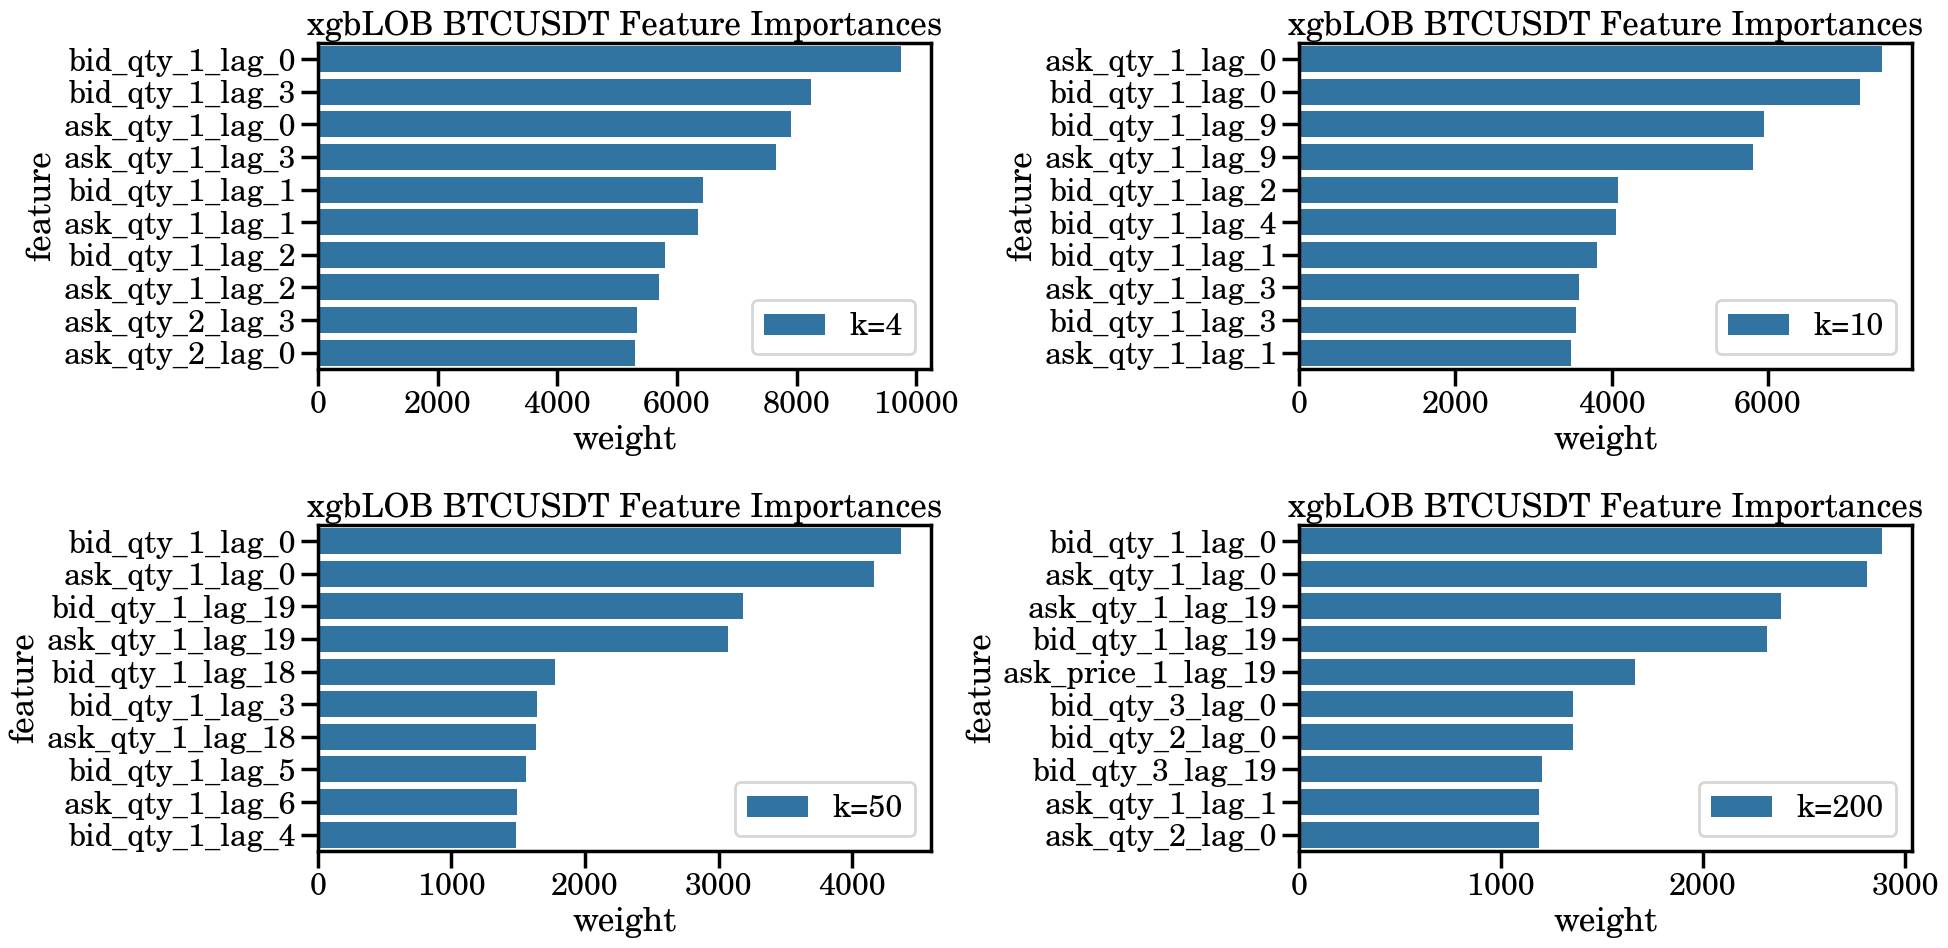
\includegraphics[width=1.0\textwidth]{./images/xgboost_LOB_BTCUSDT_top_10_feature_importances.png}
    \caption{Top 10 XGBoost LOB Feature Importances for BTCUSDT, measured by weight = number of times a feature was split on.}
    \label{top_10_lob_features}
\end{figure}
We see that for the LOB features, across all $k$, the highest weight features are 
the most current (lag 0) bid and ask quantities at the first level. This is very interesting,
and tells us that for the LOB model the most recent features are always the most relevant.
As we increase $k$, we start seeing larger lags being more important.  Recall that due to memory constraints
we set $T=10$, so the maximum lag is 9. For $k > 10$ it seems
we would certainly benefit from a larger lookback.
Also a very important note; all of the top 10 features are quantity features. Recall
that the LOB features are both quantity and price. Clearly this shows that the model
is not really using the price features at all, and this demonstrates the need for a better
representation, such as orderflow.

Next we plot the top 10 OF features for xgbOF BTCUSDT in figure \ref{top_10_of_features}.
\begin{figure}[htpb]
    \centering
    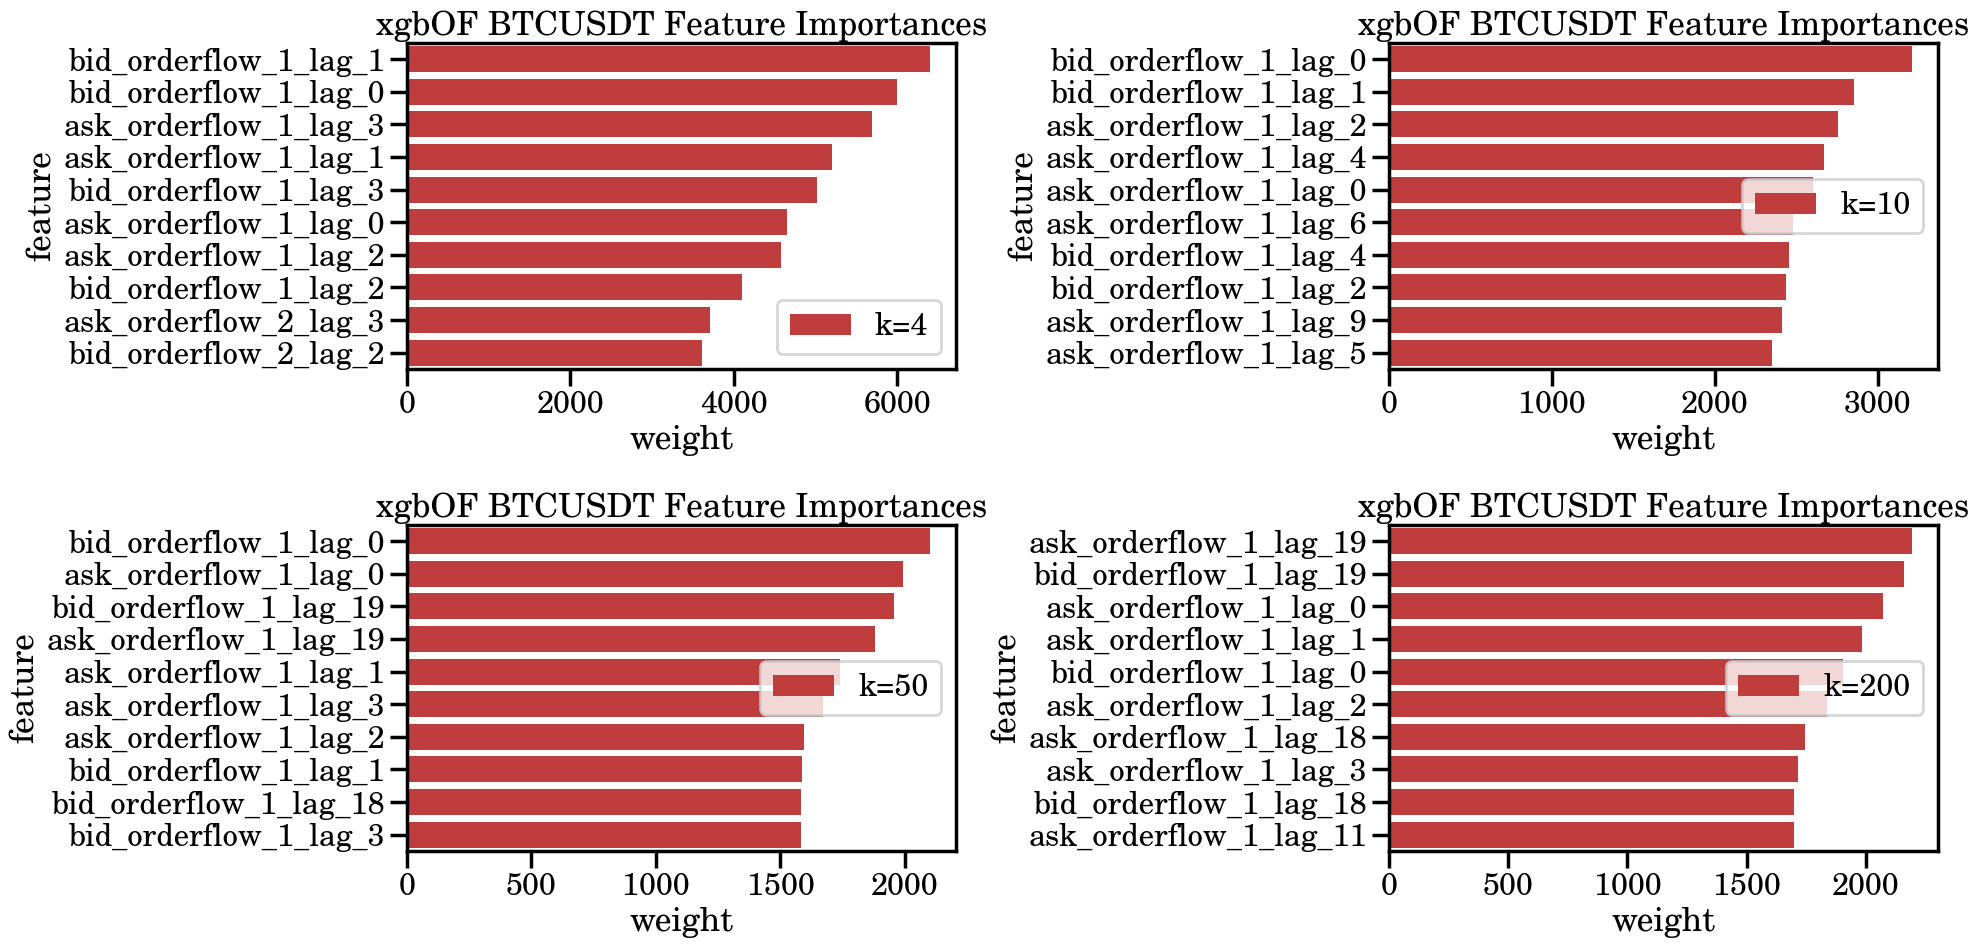
\includegraphics[width=1.0\textwidth]{./images/xgboost_OF_BTCUSDT_top_10_feature_importances.png}
    \caption{Top 10 XGBoost OF Feature Importances for BTCUSDT, measured by weight = number of times a feature was split on.}
    \label{top_10_of_features}
\end{figure}
So interestingly we see that for smaller $k$ the first level orderflow is not always the highest weighted.
We 



\begin{figure}[htpb]
    \centering
    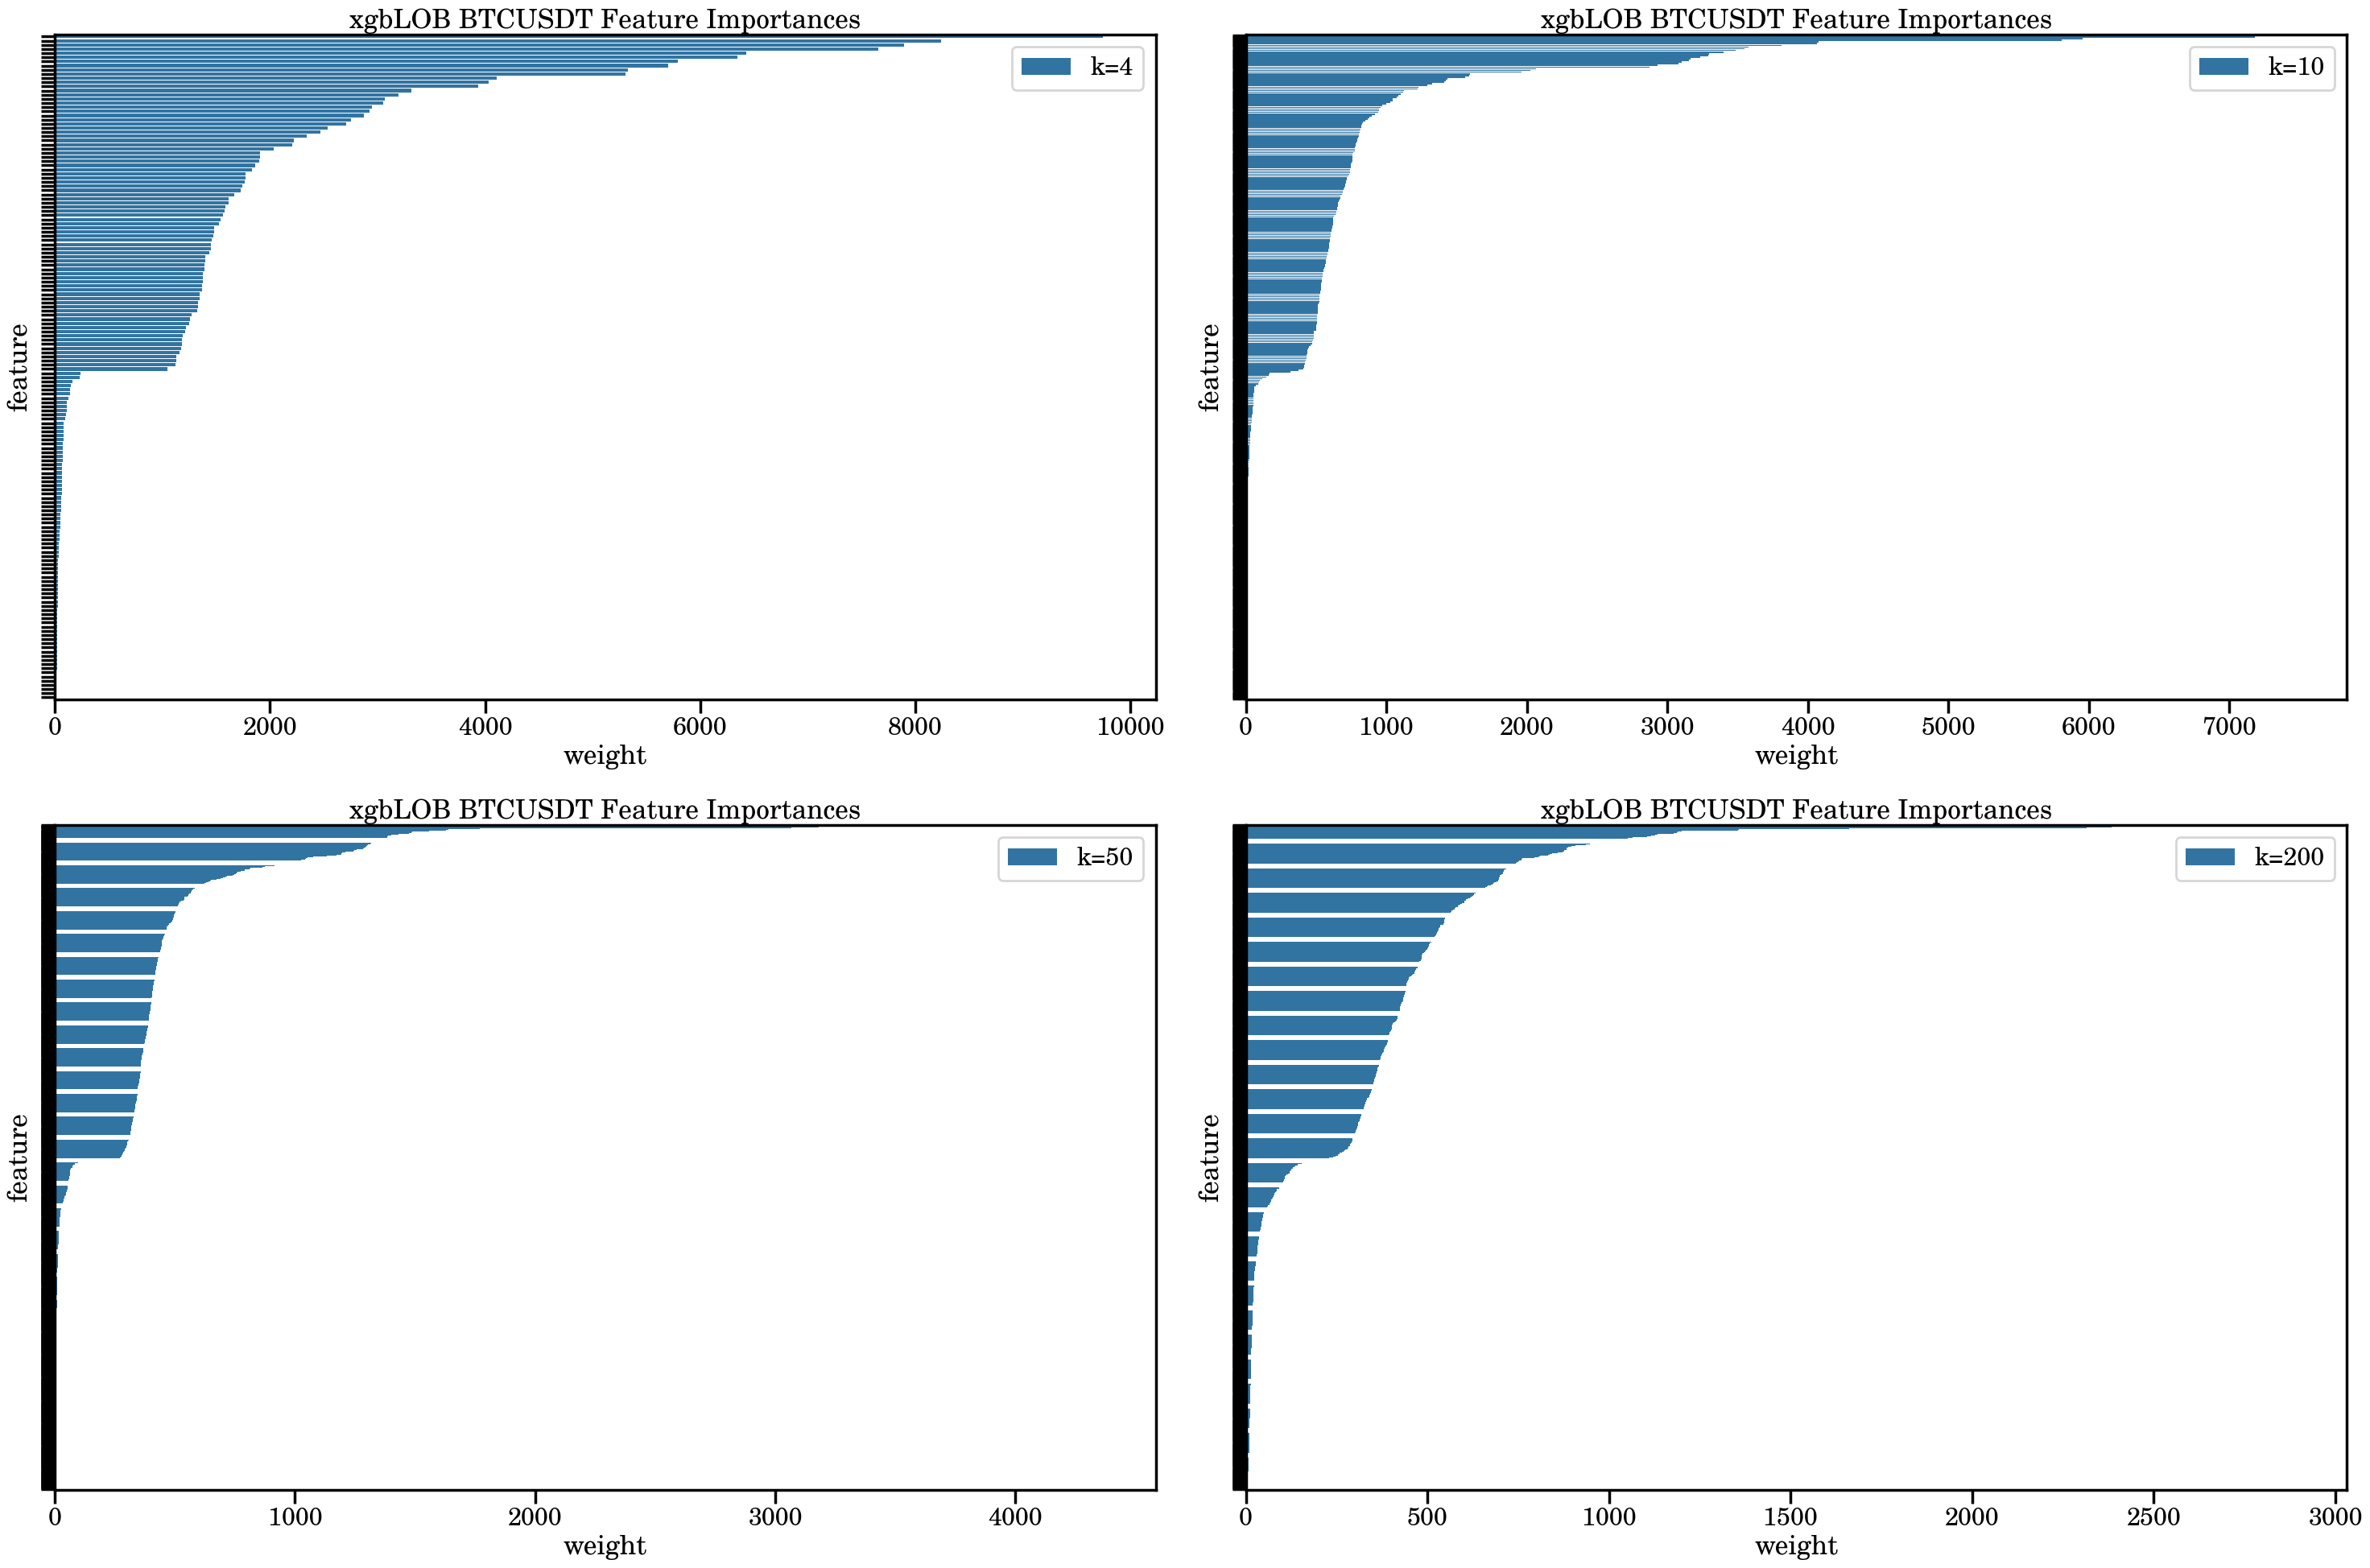
\includegraphics[width=1.0\textwidth]{./images/xgboost_LOB_BTCUSDT_all_feature_importances.png}
    \caption{}
\end{figure}

\begin{figure}[htpb]
    \centering
    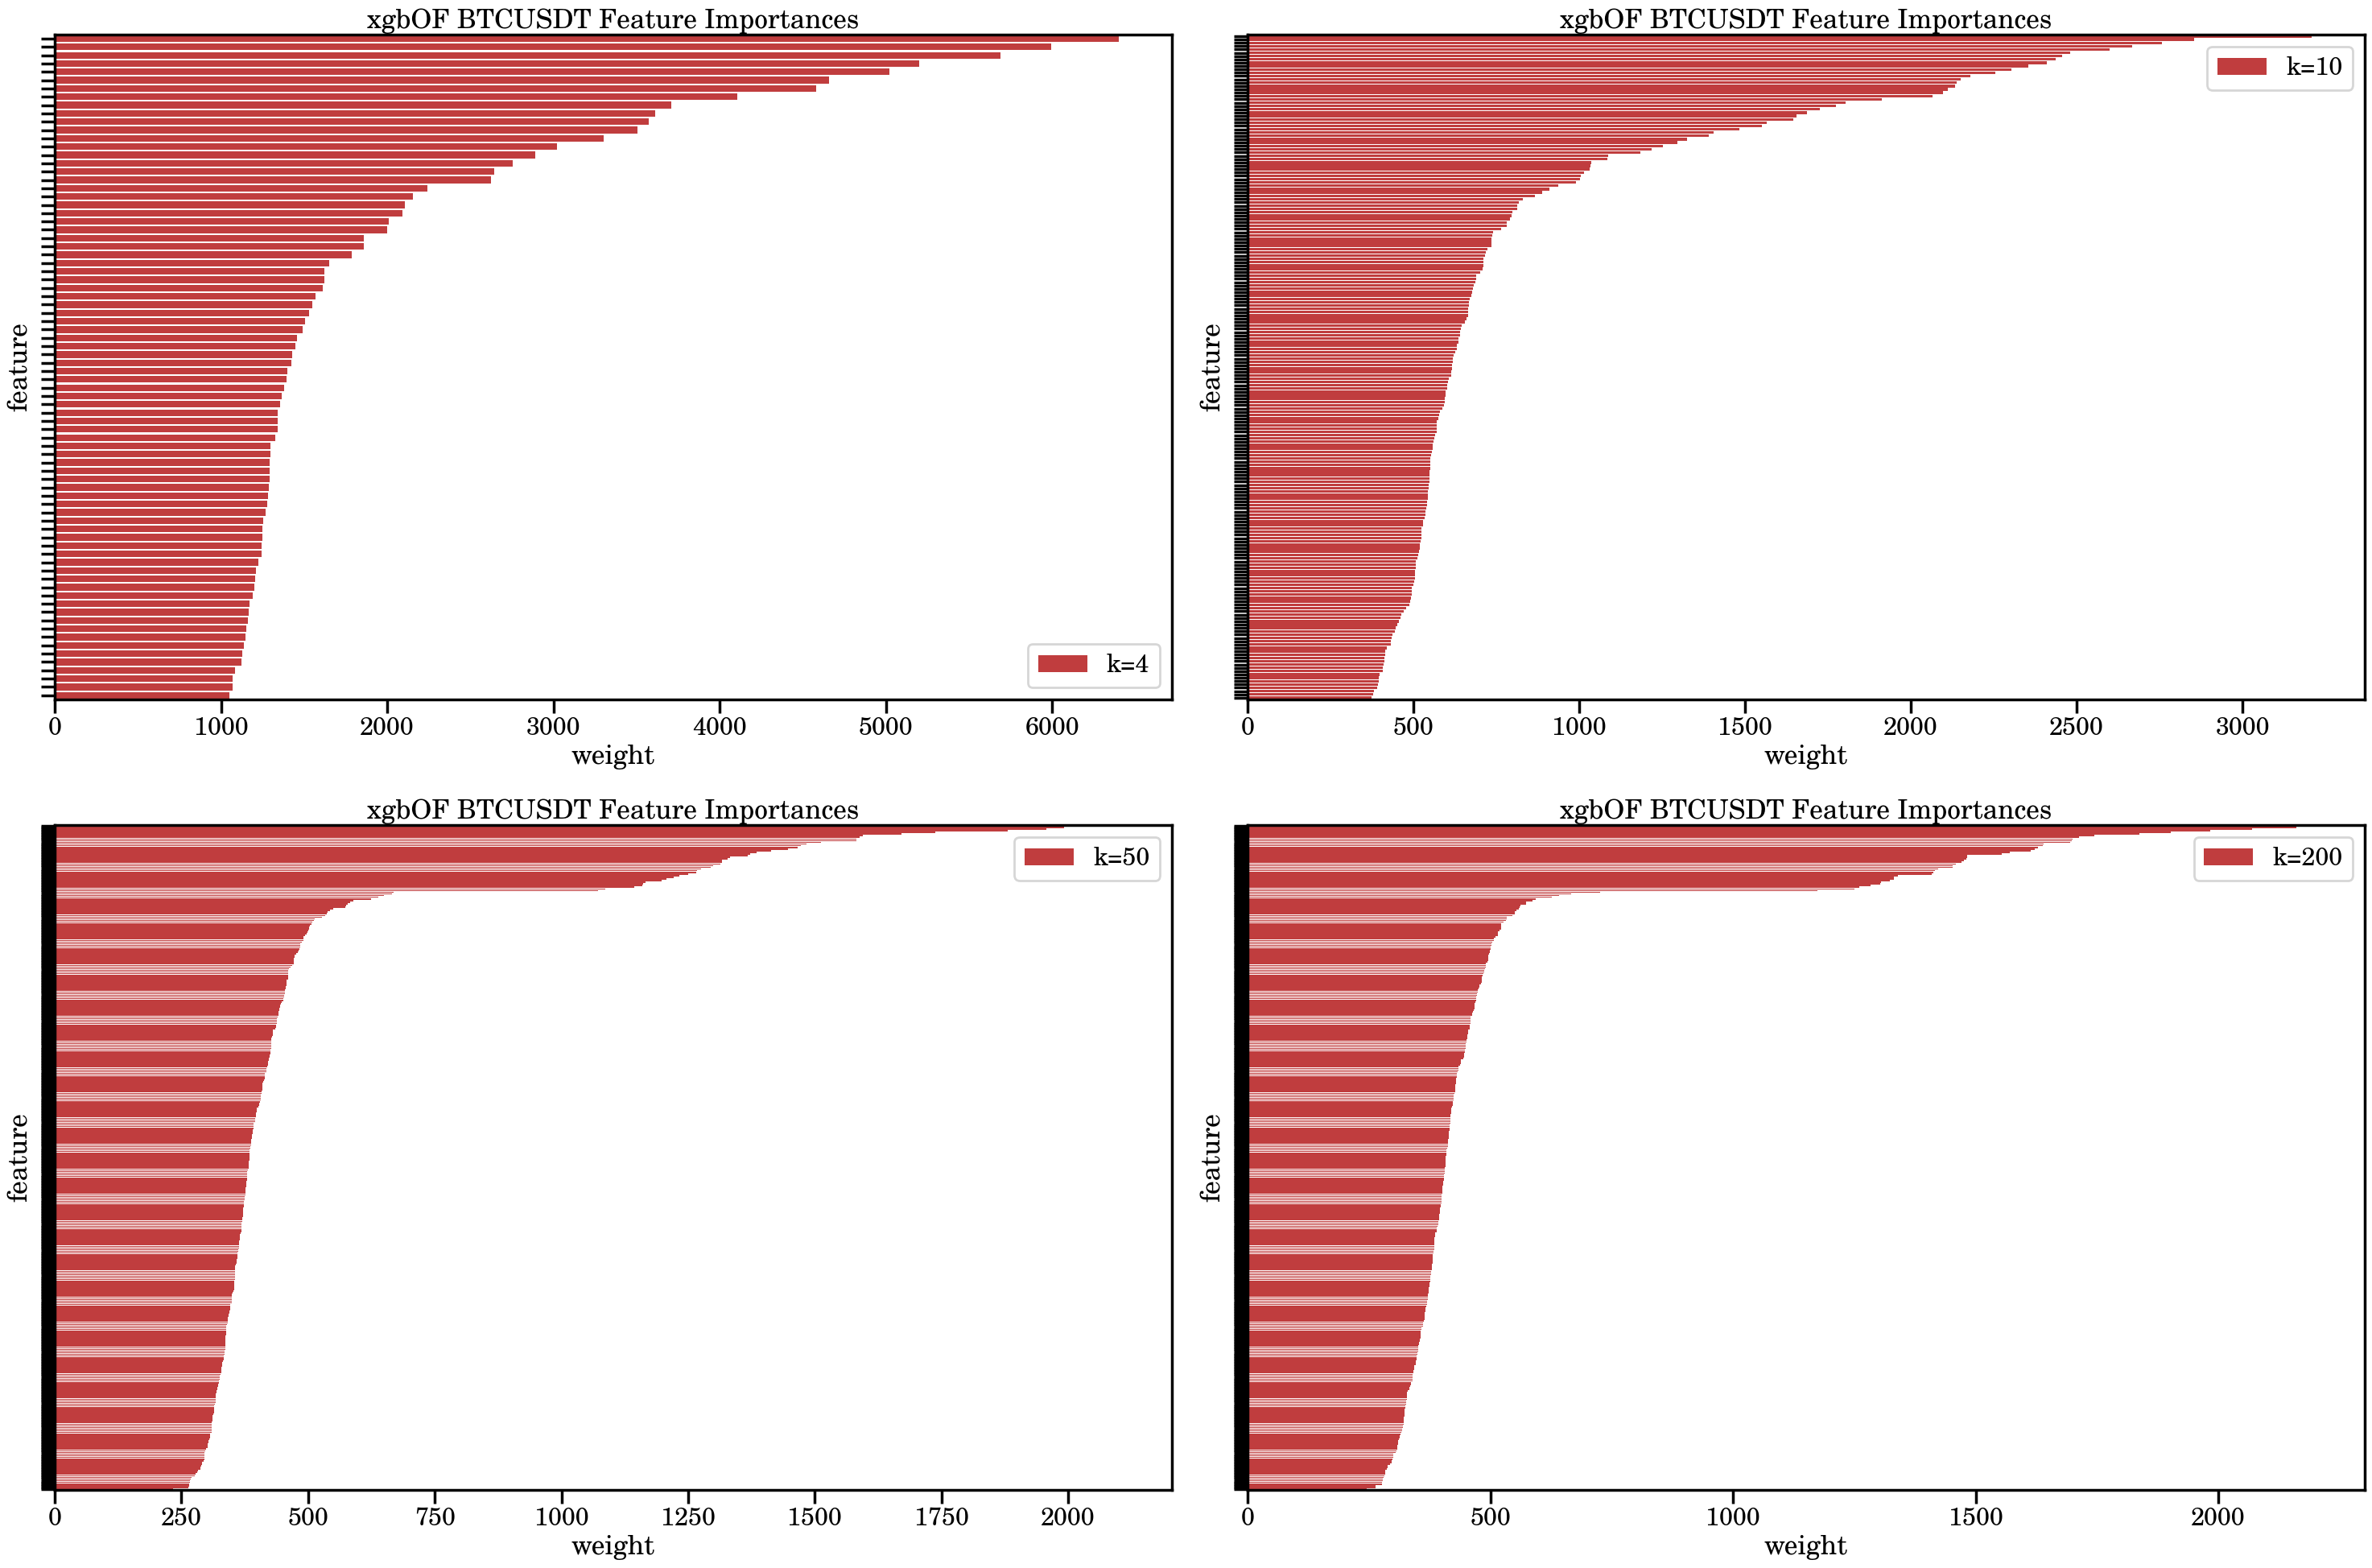
\includegraphics[width=1.0\textwidth]{./images/xgboost_OF_BTCUSDT_all_feature_importances.png}
    \caption{}
\end{figure}

\subsection{Imbalanced Classification}



\section{Conclusion}
\textbf{TODO}


\clearpage

\appendix

\chapter{Websocket Data Summary Statistics}

\chapter{Alternative Data Source}

\section{Introduction}

Initially we used the Binance historical Tick-level Orderbook API endpoint.
This returns compressed L2 representations of the orderbook going back multiple years and
for all available symbols.

The data is organized into compressed directories, one for each day. In each directory
there is a snapshot file and an updates file. The snapshot file contains all levels
of the orderbook at the start of the day. See Table \ref{table:snap} \footnote{Originally the raw data was using "b" for bids and "a" for asks in the side column, but we encode bids with $1$s and asks with $0$s so that our data is entirely numerical.}
for an example of a snapshot DataFrame.

\begin{table*}[ht!]
    \centering
    \resizebox{\textwidth}{!}{
        \begin{tabular}{|c|c|c|c|c|c|c|}
            \hline
            Row & timestamp & first\_update\_id & last\_update\_id & side & price & qty \\
            \hline
            1 & 1689033589005 & 3046269468672 & 3046269468672 & 0 & 30395.5 & 5.174 \\
            2 & 1689033589005 & 3046269468672 & 3046269468672 & 0 & 30395.6 & 0.002 \\
            3 & 1689033589005 & 3046269468672 & 3046269468672 & 0 & 30395.7 & 0.001 \\
            4 & 1689033589005 & 3046269468672 & 3046269468672 & 0 & 30395.8 & 0.001 \\
            \vdots & \vdots & \vdots & \vdots & \vdots & \vdots & \vdots \\
            100343 & 1689033589005 & 3046269468672 & 3046269468672 & 1 & 30395.0 & 0.002 \\
            100344 & 1689033589005 & 3046269468672 & 3046269468672 & 1 & 30395.1 & 0.002 \\
            100345 & 1689033589005 & 3046269468672 & 3046269468672 & 1 & 30395.2 & 0.329 \\
            100346 & 1689033589005 & 3046269468672 & 3046269468672 & 1 & 30395.3 & 0.002 \\
            \hline
        \end{tabular}
    }
    \caption{Example snapshot data for BTCUSDT.}
    \label{table:snap}
\end{table*}

The updates file contains all of the updates for the day.
Each row of the updates file represents a change to a price level or a new price level.
So the idea is to start with the snapshot, then iteratively apply the updates, row by row,
to update the state of the orderbook. For example, if a row of the updates table has quantity 0.0,
this means at that time, the corresponding price level cleared and we delete that row
from our reconstructed orderbook. So in this way we can reconstruct the orderbook at any time
by taking our snapshot and applying the updates that happened up to that time.
See Table \ref{table:updates} for an example of an updates DataFrame.



\begin{table*}[ht]
    \centering
    \resizebox{\textwidth}{!}{
        \begin{tabular}{|c|c|c|c|c|c|c|}
            \hline
            Row & timestamp & first\_update\_id & last\_update\_id & side & price & qty \\
            \hline
            1 & 1689033589005 & 3046269468673 & 3046269468673 & 1 & 30379.8 & 0.24 \\
            2 & 1689033589005 & 3046269468685 & 3046269468685 & 1 & 5000.0 & 0.648 \\
            3 & 1689033589005 & 3046269468690 & 3046269468690 & 0 & 30401.4 & 1.101 \\
            4 & 1689033589005 & 3046269468692 & 3046269468692 & 1 & 30379.9 & 0.0 \\
            \vdots & \vdots & \vdots & \vdots & \vdots & \vdots & \vdots \\
            146793483 & 1689119989003 & 3049606768393 & 3049606768393 & 1 & 5000.0 & 0.534 \\
            146793484 & 1689119989003 & 3049606768394 & 3049606768396 & 1 & 5000.0 & 0.528 \\
            146793485 & 1689119989004 & 3049606768405 & 3049606768405 & 0 & 30618.1 & 3.906 \\
            146793486 & 1689119989004 & 3049606768408 & 3049606768408 & 1 & 5000.0 & 0.53 \\
            \hline
        \end{tabular}
    }
    \caption{Example updates data for BTCUSDT.}
    \label{table:updates}
\end{table*}


\section{On Efficient Parsing}

For our purposes, we want the top $L$ best bids and asks at regular intervals, so
we have to apply the updates to the snapshots for each day and parse this data.
This is non-trivial and took some effort, so we take a small detour here to 
present our parsing algorithm and analyze it's efficiency.

This task is harder than one might think on first consideration, due to the fact
that we can't just keep track of the top $L$ levels, since the updates need to be applied
iteratively. For example, if the last price level is cleared and then the $L+1^{\text{th}}$ level
becomes the $L^{\text{th}}$ level, but we were only applying updates to the top $L$ levels,
then this level will not have been correctly updated. For this reason, we must keep track
of the state of the entire orderbook at all times.

Our algorithm initialises the reconstructed orderbook using the snapshot, then iteratively applies
the updates to the reconstructed orderbook. At regular intervals (every $\Delta t$ updates) we
then record the top $L$ best bids and asks from our reconstructed orderbook.

When applying an update, we have three cases that we have to handle:
\begin{enumerate}
    \item A new price level is instantiated.
    \item An existing price level is cleared/deleted.
    \item An existing price level is updated (quantity updated).
\end{enumerate}

For each of these cases, we determine the index in our reconstructed orderbook
where the change needs to happen, then we apply the change. In order to efficiently do this, we split our
orderbook into bids and asks and maintain a sorted ascending order.
This means we can use binary search to find the index which runs in $O(\log_2(S))$ 
where $S$ is the length of the orderbook. Also since most of the updates
happen at the top of the orderbook, if we order the bids/asks so the smallest values
are first (ascending order), then we have a very good average case runtime.
Also for consistency we want the best bid/ask to be first.
Since smaller asks are better, this just means we have to sort our asks in 
ascending order. For bids we have the issue that higher bids are better,
so we could use branching if statements here but this is inefficient for a large
number of iterations, so instead we use a trick. We sort the bids in descending order,
so that the best bid is first, and then we multiply the prices by -1, so that
the smallest values are first. This leads to very fast runtimes in practice.

Once we have found this index, we either insert the update, delete the row or
update an existing row.

Every $\Delta t$ updates, we store the top $L$ best bids and asks from our reconstructed
orderbook in a DataFrame, which is then returned once all the updates
have been applied. Since we know the number of updates and also $\Delta t$, we can
pre-allocated this DataFrame with $\lceil \text{length(updates)} / \Delta t \rceil + 1$ rows\footnote{+1 is for the initial snapshot, t=0 case.}, so that
adding a record is only $O(1)$. 

See Algorithm \ref{algo:levels} for the pseudocode.

\section{The Parsing Algorithm}


\begin{algorithm*}
\caption{reconstruct\_orderbook}
\begin{algorithmic}[1]
\Function{reconstruct\_orderbook}{$L$::Int, $\Delta t$::Int, snap::DataFrame, updates::DataFrame}
    \State asks $\gets$ snap[side == 0, :]
    \State bids $\gets$ snap[side == 1, :]
    \State sort!(bids, by=price, ascending=false) \Comment{Best bid/ask in first row}
    \State bids[:, price] *= -1.0 \Comment{Trick so we have ascending order}
    \State $N \gets$ $\lceil \text{length(updates)} / \Delta t \rceil+ 1$ \Comment{+ 1 for initial snapshot row}
    \State top\_bids $\gets$ bids[1:L, :] \Comment{Initial case}
    \State top\_asks $\gets$ asks[1:L, :]
    \State levels $\gets$ zeros($N$, $1 + 4L$)  \Comment{Pre-allocate our parsed levels}
    \State levels[1, :] $\gets$ concat([ \Comment{Initial edge case} \\
    \hspace{35pt}  snap[1, timestamp], \\
    \hspace{35pt}  top\_bids[:, price] * -1.0, \\
    \hspace{35pt}  top\_asks[:, price],\\
    \hspace{35pt}  top\_bids[:, qty],\\
    \hspace{35pt}  top\_asks[:, qty]\\
    \hspace{16pt}])
    \State levels\_idx $\gets 2$
    \For{(t, update) in \text{enumerate}(updates)} \Comment{Iterate over each row of updates}
        \If{update.side == 1}
            \State orderbook $\gets$ bids  \Comment{orderbook is a reference not a copy}
            \State update.price *= -1  \Comment{Trick so we have descending order}
        \Else
            \State orderbook $\gets$ asks
        \EndIf
        \State insert\_idx $\gets$ searchsortedfirst(orderbook[:, price], update.price)
        \If{insert\_idx $>$ nrow(orderbook) or orderbook[insert\_idx, price] $\neq$ update.price}
            \State insert!(orderbook, insert\_idx, update) \Comment{Case 1: New price}
            \ElsIf{update.qty $== 0.0$} \Comment{Case 2: Deleting a price}
            \State deleteat!(orderbook, insert\_idx)

            \Else  \Comment{Case 3: Updating the quantity for a price}             
            \State orderbook[insert\_idx, :] $\gets$ update
        \EndIf \\

        
        \If{$t ~ \% ~ \Delta t == 0$} \Comment{Record the state of the top L levels every $\Delta t$ updates.}
            \State top\_bids $\gets$ bids[1:L, :]
            \State top\_asks $\gets$ asks[1:L, :]
            \State levels[levels\_idx, :] $\gets$ concat([ \\
            \hspace{65pt}    update.timestamp, \\
            \hspace{65pt}  top\_bids[:, price] * -1.0, \\
            \hspace{65pt}  top\_asks[:, price],\\
            \hspace{65pt}  top\_bids[:, qty],\\
            \hspace{65pt}  top\_asks[:, qty]\\
            \hspace{47pt}])
            \State levels\_idx += 1
        \EndIf
    \EndFor
    \State \Return levels
\EndFunction
\end{algorithmic}
\label{algo:levels}
\end{algorithm*}

\section{Complexity Analysis}



If we denote $U$ to be the number of updates and $S$ to be the size of the initial snapshot/number of levels
in our reconstructed orderbook (on average this should be roughly constant). Then we see that 
Algorithm \ref{algo:levels} has $O(US)$ worse case runtime complexity, since for each of the $U$ 
updates, we searchsorted through our reconstructed orderbook, which runs in $O(\log_2(S))$ worst case,
and then either delete, insert or update a price level. Inserting and deleting are both $O(S)$ worst case,
but updating is only $O(1)$, so worst case we have $O(\log_2(S) + S) = O(S)$  time complexity per
iteration. So in total we have $O(US)$ worst case time complexity. Then we also have $O(U + S)$ memory
complexity since we store the updates and reconstructed orderbook in memory at all times. 
In practice we can use a RecordCursor object, to efficiently read the updates line by line, instead
of having to load them into memory all at once. This reduces the memory complexity down to $O(S)$.

Note that $U \gg S$ and so for efficiency we mostly care about the complexities in terms of $U$. 

For our data we observe $U \approx 1.5 \times 10^3 S$ which is a pretty massive difference.

So we see that we achieve linear worst case time complexity in $U$ and due to the
sequential nature of the updates, this is clearly the best possible time complexity for 
this problem. We verify the linear time complexity experimentally in Figure \ref{complexity}

\begin{figure*}[htpb]
    \centering
    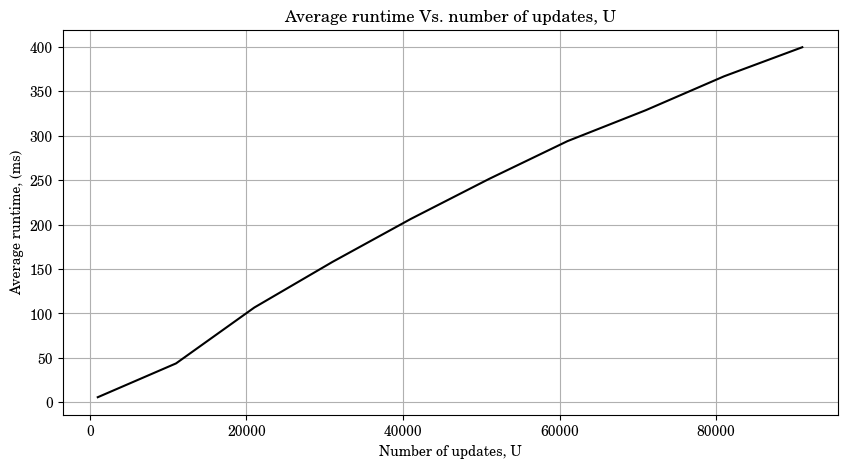
\includegraphics[width=1.0\textwidth]{./images/complexity.png}
    \caption{reconstruct\_orderbook runtime as a function of the number of updates, $U$.\\ Note that the runtimes are recorded 100 times and then averaged.}
    \label{complexity}
\end{figure*}

\section{Data Issues}

We can apply our algorithm to each day of data and then combine the results.
In order to check our data, we parse the data for several months in 2023 of BTCUSDT data 
and then compare to a reference.

For our reference, we have access to hourly BTCUSDT mid prices from an undisclosed source,
going back 1 year.

We resample our parsed data to an hourly resolution and then calculate hourly mid prices.
We plot our parsed data against the reference data in Figure \ref{missing}.

Unfortunately we find that there is a lot of missing data and we verify that this
is from the underlying raw data and not an issue with our parsing.

Due to this, we are unable to use this historical data for our purposes.


\begin{figure*}[htpb]
    \centering
    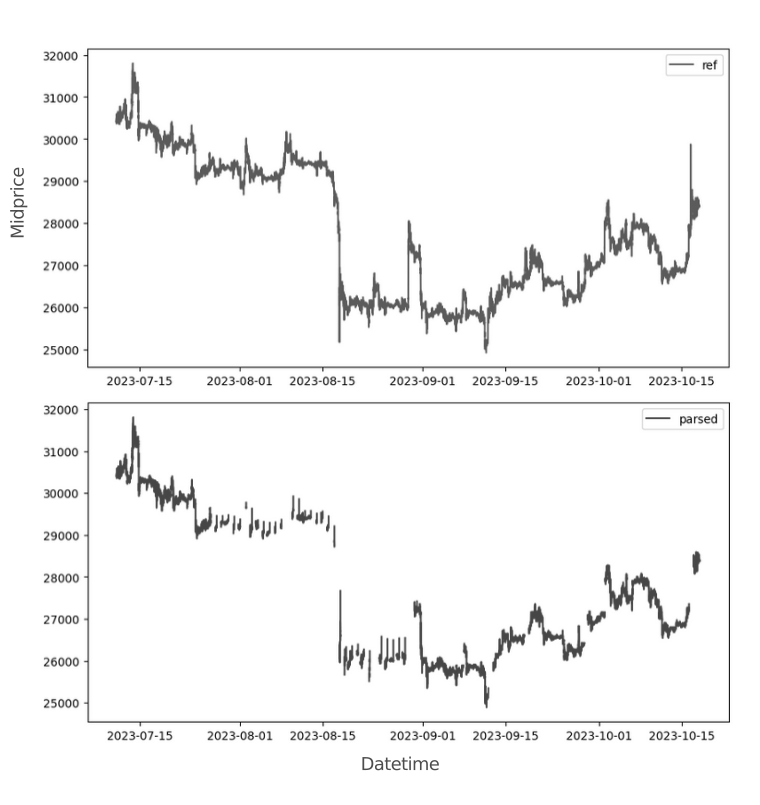
\includegraphics[width=1.0\textwidth]{./images/parsed.png}
    \caption{Reference hourly mid prices (top) Vs. parsed mid prices (bottom). Observe the general shape is correct, however
    there are large gaps due to missing data.}
    \label{missing}
\end{figure*}

\chapter{Application of the Hasbrouck Information Share}

\section{The Hasbrouck Information Share}
In any market we constantly have new information/events that determine prices. This is often called "price discovery".

Price discovery is defined to be the process by which new information is incorporated into
market prices.

Suppose we have multiple price series that are based on the same underlying security, then by arbitrage these prices should not diverge significantly, since they share the same underlying stochastic factor(s).

\cite{HASBROUCK1995} refers to the shared stochastic factor as the "implicit efficient price".
This is the source of long-term permanent price change.
It assumed that each price series shares the same random walk component and that each series also has zero-mean i.i.d disturbances that are uncorrelated. 
These disturbances affect the price series movement in the short term, but often these
"innovations" will also have a permanent affect on the long term shared implicit efficient price. For example if we have BTC trading on FTX and Binance, then when the news hits
that FTX has is shutting down this will cause a temporary shock in the FTX BTC price,
that will eventually impact all other BTC markets.

The idea behind Hasbrouck's Information Share is to estimate what proportion of the long-term variance in the shared implicit efficient price can be attributed to innovations from the respective price series.

So formally, we start with a price series: $p_{t} := (p_{1t}, p_{2t}, \dots, p_{nt})^T \in \mathbb{R}^n$ where $p_{it}$ represent
individual price series which all share the same common stochastic factor (random walk component). So these series are all co-integrated $I(1)$.

\cite{HASBROUCK1995} converts this price series into a Vector Error Correction Model or VECM for short:
\begin{equation}
    \Delta p_{t} = \alpha \beta' p_{t-1} + \sum_{i=1}^k \Gamma_{i} \Delta p_{t-i} + e_{t} \in \mathbb{R}^n
\end{equation}
The first term models the long-term interaction between the different price series. The second term models the short term dynamics of each series and the final $e_{t}$ represents the innovations.

\cite{HASBROUCK1995} then re-formulates the VECM as a Vector Moving Average of VMA model:
\begin{equation}
    \Delta p_{t} = \Psi(L)e_{t} \label{VMA}
\end{equation}
This has integrated form:
\begin{equation}
    p_{t} = \Psi(1) \sum_{s=1}^t e_{s} + \Psi^*(L)e_{t}
\end{equation}
where $\Psi(L), \Psi(1), \Psi^*(L)$ are matrix polynomials in the lag operator $L$ and
\begin{equation}
    \Psi(1) = I_{n} + \sum_{t=1}^\infty \Psi_{t} \label{Psi1}
\end{equation}
So the vector $\Psi(1)e_{t}$ represents the long run impact of the innovation $e_{t}$ on each price series.

The fact that $\beta' p_{t}$ is stationary implies that $\beta' \Psi(1) = 0$ and then by construction of $\beta'$ we have that all rows of $\Psi(1)$ should be identical. In other words, we expect the long run impact
on each price series to be approximately the same. We denote the common row vector
of $\Psi(1)$ as $\psi$. So $\psi e_{t}$ gives us the component of the price change that is permanently affected by the innovation $e_{t}$. Note that:
\begin{equation}
    \text{var}(\psi e_{t}) = \psi \Omega \psi'
\end{equation}
Where we have defined $\Omega := \text{cov}(e) \in \mathbb{R}^{n \times n}$, where $e = [e_{1}; e_{2}; \dots; e_{T}]' \in \mathbb{R}^{T \times n}$
Then the variance attributed to an individual price series $j$ is given by $\psi_{j}^{2} \Omega_{jj}$ and so we arrive at the Hasbrouck Information share:
\begin{equation}
    S_{j} := \frac{\psi_{j}^{2} \Omega_{jj}}{\psi \Omega \psi'} \label{Hasequation}
\end{equation}
However as \cite{HASBROUCK1995} points out, if the innovations are not un-correlated across price series, then $\Omega$ will not be diagonal and this measure won't make sense.

So the Cholesky decomposition is used to try and alleviate the contemporary correlations.
Decompose $\Omega$ as:
\begin{equation}
    \Omega = F F'
\end{equation}
where $F$ is a lower triangular matrix. Then we can attain an upper/lower bound on the
information share $j$ when the price series $j$ is first/last in $p_{t}$, with:
\begin{equation}
    S_{j} = \frac{([\psi F]_{j})^{2}}{\psi \Omega \psi'}
\end{equation}

To estimate $\Psi(1)$, we turn to the work of \cite{KARABIYIK2022} who derive the following estimators:

\begin{align}
\beta' &:= [1_{(n-1)}; -I_{(n-1)}] \in \mathbb{R}^{(n-1) \times n} \\
\hat{\alpha} &:= \Delta p' M_{x} p_{-1}^* [ (p_{-1}^*)' M_{x} p_{-1}^*]^{-1} \in \mathbb{R}^{n \times (n-1)}\\
\Delta p &:= [\Delta p_{1}; \dots ; \Delta p_{T}]' \in \mathbb{R}^{T \times n} \\ 
p_{-1}^* &:= [\beta' p_{0}; \dots ; \beta' p_{T-1}]' \in \mathbb{R}^{T \times (n-1)} \\
&= [p_{0}; \dots ; p_{T-1}]' \beta \\
M_{x} &:= I_{T} - X(X'X)^{-1} X' \in \mathbb{R}^{T \times T} \\
X &:= [\Delta p_{-k}; \dots ; \Delta p_{-1}] \in \mathbb{R}^{T \times kn} \\
\Delta p_{-l} &:= [\Delta p_{1-l}; \dots ; \Delta p_{T-l}]' \in \mathbb{R}^{T \times n} \\
\hat{e} &:= M_{x}(\Delta p - p^{*}_{-1} \hat{\alpha}') \in \mathbb{R}^{T \times n}\\
\hat{\Omega} &:= \frac{1}{T} \hat{e}' \hat{e} \in \mathbb{R}^{n \times n}
\end{align}

Then they also derive a consistent estimator for $\alpha_{\perp} \in \mathbb{R}^{n \times 1}$ by taking the only eigenvector of $M_{\hat{\alpha}} := I_{n} - \hat{\alpha}(\hat{\alpha}' \hat{\alpha})^{-1} \hat{\alpha}'$ with eigenvalue $1$. (Normalized to have norm $1$).
Following \cite{HASBROUCK1995}, they also take the Cholesky decomposition of $\hat{\Omega}$ to get $\hat{F}$.
(We refer the interested reader to \cite{KARABIYIK2022} for derivation and proofs of these estimators).

So using these estimators we arrive at an estimator for the information share of the $j^{th}$ price series:

\begin{equation}
    \hat{IS}_{j} := \frac{([ \hat{\alpha}_{\perp}'\hat{F}]_{j})^2}{\hat{\alpha}_{\perp}' \hat{\Omega} \hat{\alpha}_{\perp}}
\end{equation}

As \cite{HASBROUCK1995} points out, the ordering of the price series will have an effect on the information share, so to achieve upper/lower bounds on information share for price series $j$, we permute the $p$ so that the $p_{j, t}$ is first/last.


\section{A Toy Example}
We demonstrate this methodology with a synthetic example.

Suppose we have two price series, with the first being modelled as a simple random walk
and the second modelled as a lagged version of the first, with some extra randomness introduced.

\begin{align}
    p_{1, t} &= p_{1, t-1} + w_{1, t} = w_{1, t} + w_{1, t-1} + \sum_{s=1}^{t-2} w_{1, s} \label{toy1}\\
    p_{2, t} &= p_{1, t-2} + w_{2, t} = w_{2, t} + \sum_{s=1}^{t-2} w_{1, s} \label{toy2}
\end{align}

Where $w_{j, t} \sim N(0, 1)$ i.i.d and $p_0 := 0$.

We can clearly verify that this example is co-integrated $I(1)$.

This could represent two different markets, each with their own news shocks/innovations
where the second market reacts to the first market price changes. So in this
situation we would have an information share of $1$ for the first market and $0$ for the
second market, since the first market completely drives price discovery.

\begin{figure*}[htpb]
    \centering
    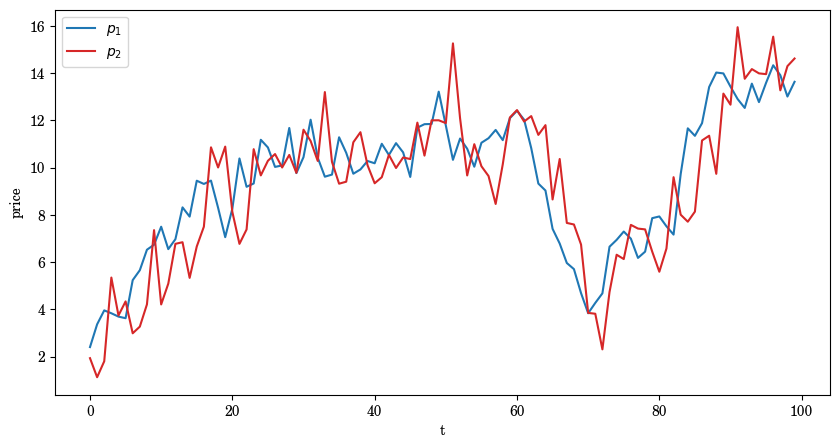
\includegraphics[width=1.0\textwidth]{./images/lagged_walk.png}
    \caption{Lagged random walks. Clearly we see $p_2$ lags behind $p_1$. Note that we only plot $t$ up to 100 for visual clarity.}
\end{figure*}

We derive this result analytically in the following.

Using (\ref{toy1}) and (\ref{toy2}) we get:
\begin{align*}
    \Delta p_{1, t} &= w_{1, t} \\
    \Delta p_{2, t} &= w_{1, t-2} + w_{2, t} - w_{2, t-1}
\end{align*}

Then we can convert to the VMA representation given in (\ref{VMA}):
\[
    \underbrace{
    \begin{bmatrix}
    w_{1,t} \\
    w_{1,t-2} + w_{2,t} - w_{2,t-1}
    \end{bmatrix} 
    }_{= \Delta p}
    =
    \underbrace{
    \begin{bmatrix}
    1 & 0 \\
    L^{2}  & 1 - L
    \end{bmatrix}
    }_{= \Psi(L)}
    \underbrace{
    \begin{bmatrix}
    w_{1,t} \\
    w_{2,t}
    \end{bmatrix}
    }_{=e_t}
.\]

Then recalling that $\Psi(L) = \sum_{k=0}^{\infty} \Psi_k L^k$ 
we have the coefficients:
\begin{align*}
    \Psi(L) =
\underbrace{
\begin{bmatrix}
1 & 0 \\
0 & 1
\end{bmatrix}
}_{:= \Psi_0} L^0
+
\underbrace{
\begin{bmatrix}
0 & 0 \\
0 & -1
\end{bmatrix}
}_{:= \Psi_1} L^1
+
\underbrace{
\begin{bmatrix}
0 & 0  \\
1 & 0
\end{bmatrix}
}_{:= \Psi_2}L^{2}
\end{align*}
Then plugging these into (\ref{Psi1}) we get:
\[
    \Psi(1) = \begin{bmatrix} 1 & 0 \\ 1 & 0 \end{bmatrix} 
.\]
Which has common row vector $\psi := [1 ~ 0]$. Then using (\ref{Hasequation})
and $\Omega = I_2$ we get the Information Share of the first price series to be $1$
and the Information Share of the second series to be $0$, as expected.

% We also examine the case when we have two simple random walks:
%
% \begin{align}
%     p_{1, t} &= p_{1, t-1} + w_{1, t} = \sum_{s=1}^{t} wShare{1, s}\\
%     p_{2, t} &= p_{2, t-1} + w_{2, t} = \sum_{s=1}^{t} w_{2, s}
% \end{align}
%
% \textbf{TODO:} Analytically derive hasbrouck information share for this example.
%
% Where $w_{j, t} \sim N(0, 1)$ i.i.d and $p_0 := 0$.
%
% Clearly this example is co-integrated $I(1)$, since $\mathbb{E}(p_{j,t}) = \sum_{s=1}^{t} \mathbb{E}(w_{j,s}) = 0$ and
% $\text{var}(p_{j, t}) = \sum_{s=1}^{t} \text{var}(w_{j, s}) = t$
% and therefore $\mathbb{E}(\Delta p_t) = \text{var}(\Delta p_t) = 0$.
%
%
% \begin{figure}[htpb]
%     \centering
%     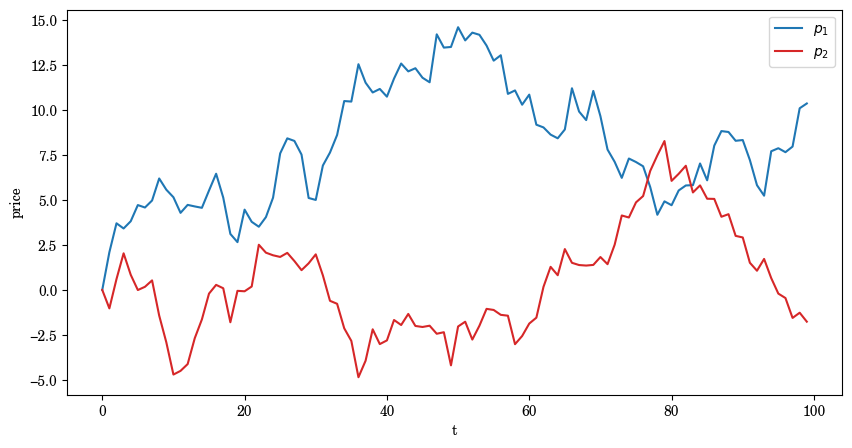
\includegraphics[width=1.0\textwidth]{./images/random_walk.png}
%     \caption{Random walks}
% \end{figure}
%
\section{Orderbook Application}

Following \cite{CAO2009} we resample our data to $1s$ intervals and define the weighted price as:
\begin{equation}
    \text{WP}^{n_{1}, n_{2}} := \frac{\sum_{j=n_{1}}^{n_{2}} q_{j}^B p_{j}^B + q_{j}^A p_{j}^A}{\sum_{j=n_{1}}^{n_{2}} (q^B_{j} + q^A_{j})}
\end{equation}
where $n_{1} \leq n_{2}$. When $n_{1} = n_{2} = 1$ we have the weighted mid price:
\begin{equation}
    \text{WP}^{1,1} = \frac{q_{1}^B p_{1}^B + q_{1}^A p_{1}^A}{q_{1}^B + q_{1}^A}
\end{equation}

So $\text{WP}^{n_{1},n_{2}}$ is an average price between level $n_{1}$ and $n_{2}$, weighted by volume, encapsulating all the information in the orderbook between levels $n_{1}$ and $n_{2}$ inclusive.

We compare the information content of $\text{WP}^{1,1}$ and $\text{WP}^{2,10}$, i.e how does the information
at the top of the book compare to the other, deeper levels.
So our price series is given by $p_t := (\text{WP}^{1,1}_t, \text{WP}^{2,10}_t)$.
The mid price and the weighted price have the same common stochastic factor,
are both non-stationary and therefore it is clear that they are $I(1)$ co-integrated.

\begin{figure*}[htpb]
    \centering
    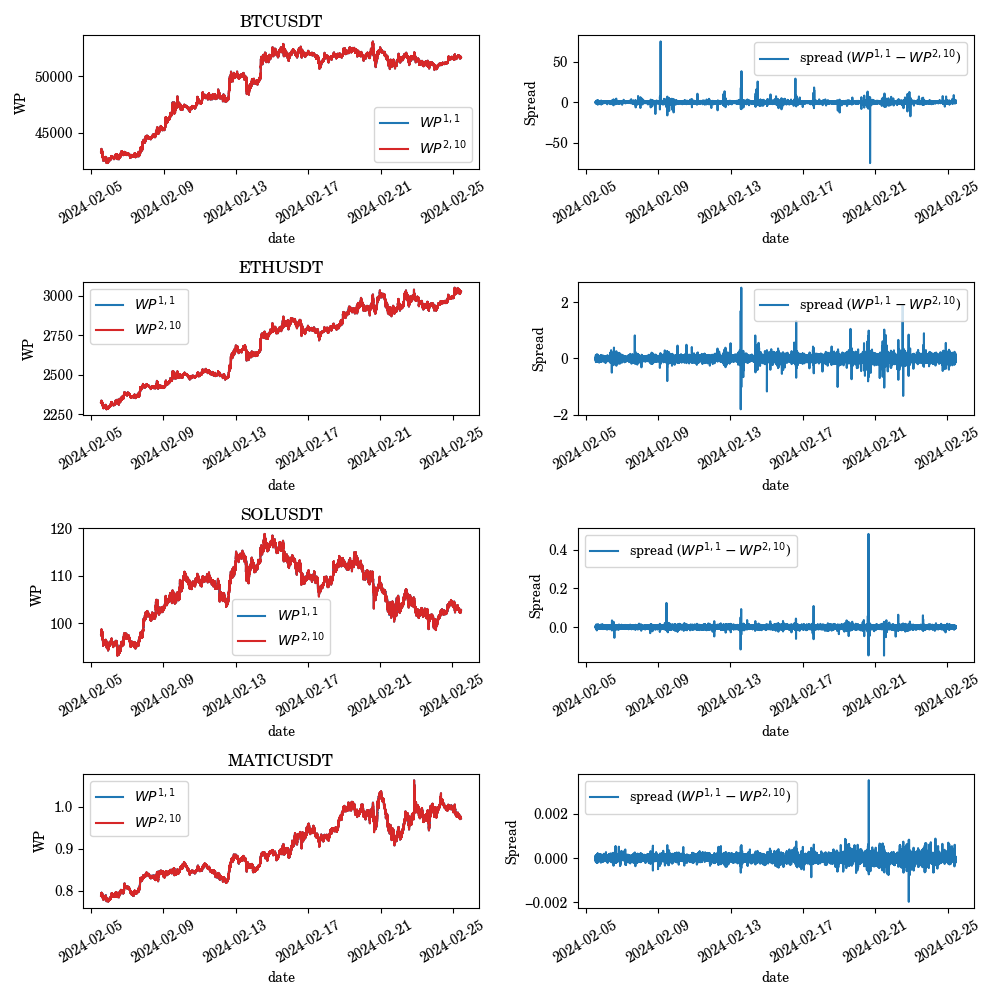
\includegraphics[width=1.0\textwidth]{./images/weighted_prices.png}
    \caption{Weighted prices and their spread for each symbol.}
    \label{spread}
\end{figure*}

Interestingly we see from Figure \ref{spread} that for our data BTCUSDT
has some very large outlier spreads whereas MATICUSDT seems to be much more stable.
Also we observe that in general across all our symbols there is a slight increase
in spread towards the end of the month.


So now we calculate \footnote{Note that when calculating information shares, we have too much data to fit
into memory, so we calculate the information share for windows of size 10,000 and then
we average. Standard deviations are also given in parenthesis.} the Information Share using the estimators we defined above
and report the results in Table \ref{table:1}.

\begin{table*}[ht!]
    \begin{center}
        \begin{tabular}{|c|c|c|c|c|}
            \hline
            Symbol    & $\text{WP}^{1,1}$ Min IS & $\text{WP}^{1,1}$ Max IS & $\text{WP}^{2,10}$ Min IS & $\text{WP}^{2,10}$ Max IS \\
            \hline
            BTCUSDT   & 0.05 (0.04)  & 0.97 (0.02)   & 0.03 (0.02) & 0.95 (0.04)   \\
            ETHUSDT   & 0.06 (0.05)  & 0.98 (0.03)   & 0.02 (0.03) & 0.94 (0.05)  \\
            SOLUSDT   & 0.08 (0.05)     & 0.98 (0.02)  & 0.02 (0.02) & 0.92 (0.05)   \\
            MATICUSDT &   0.04 (0.06)    & 0.87 (0.12)  & 0.13 (0.12) & 0.96 (0.06)  \\
            \hline
        \end{tabular}
        \caption{IS Results for each symbol.}
    \label{table:1}
    \end{center}
\end{table*}

So we see that for each price series the minimum IS is close to zero and the maximum is close 1.
This is unexpected. For example when \cite{CAO2009} applied the same methodology they
had a much tighter spread between max and min information share for each stock.
This large difference means that for us information share is hard to interpret and 
is perhaps not as useful for this application as one would have hoped.
As \cite{YAN2010} points out, large differences in minimum and maximum Information Share
occur when the residuals, $e_t$ are highly correlated across series.

When we examine our estimated $\Omega$ covariance matrices we find this to be the case.
This implies that the innovations at the top of the orderbook are highly correlated
with the innovations affecting prices further down the orderbook. As \cite{KARABIYIK2022}
points out, these correlations can be partly alleviated by using higher frequency data.
We re-sample our data to 250ms intervals (instead of 1s) and observe a reduction
in covariance. However this reduction is not sufficient and we still observe a large gap in max and min Information Shares.
This is perhaps due to the fact that
for cryptocurrency data the trading is much higher volume and higher frequency
than traditional stocks as studied in \cite{CAO2009}, and so in order for the 
innovations to be uncorrelated, we need much higher frequency sampling.
Since we are limited by our Websocket data to a minimum resolution, we can go no further. 

We conclude that for Binance Websocket data, information shocks
driving price change are highly correlated across orderbook levels.
A consequence of this being that the Hasbrouck Information Share cannot be applied reliably
to measure Information Shares across levels.


\section{DeepLOB Detailed Model Architecture}

\begin{table*}[ht]
        \centering
    \resizebox{1.0\textwidth}{!}{
            \begin{tabular}{|l|l|l|}
                \hline
                \textbf{Layer Type} & \textbf{Parameters} & \textbf{Details} \\
                \hline
                \textbf{Conv 1} & & \\
                \quad Conv2d & $1 \times 2$, 32 filters, stride $1 \times 2$ & Spatial aggregation of price and volume for each level and side.\\
                \quad LeakyReLU & negative slope = 0.01 & Activation function.\\
                \quad BatchNorm2d & 32 features & Normalization.\\
                \quad Conv2d & $4 \times 1$, 32 filters & Temporal aggregation of price and volume for each level and side.\\
                \quad LeakyReLU & negative slope = 0.01 & \\
                \quad BatchNorm2d & 32 features & \\
                \quad Conv2d & $4 \times 1$, 32 filters & Temporal aggregation of price and volume for each level and side.\\
                \quad LeakyReLU & negative slope = 0.01 & \\
                \quad BatchNorm2d & 32 features & \\
                \hline
                \textbf{Conv 2} & & \\
                \quad Conv2d & $1 \times 2$, 32 filters, stride $1 \times 2$ & Spatial aggregation of imbalance information across sides for each level.\\
                \quad Tanh & & Activation function.\\
                \quad BatchNorm2d & 32 features & \\
                \quad Conv2d & $4 \times 1$, 32 filters & Temporal aggregation of imbalance information across time for each side and level.\\
                \quad Tanh & & \\
                \quad BatchNorm2d & 32 features & \\
                \quad Conv2d & $4 \times 1$, 32 filters & Temporal aggregation of imbalance information across time for each side and level.\\
                \quad Tanh & & \\
                \quad BatchNorm2d & 32 features & \\
                \hline
                \textbf{Conv 3} & & \\
                \quad Conv2d & $1 \times 10$, 32 filters & Spatial aggregation of imbalance information across all levels.\\
                \quad LeakyReLU & negative slope = 0.01 & \\
                \quad BatchNorm2d & 32 features & \\
                \quad Conv2d & $4 \times 1$, 32 filters & Temporal aggregation of imbalance information across all levels.\\
                \quad LeakyReLU & negative slope = 0.01 & \\
                \quad BatchNorm2d & 32 features & \\
                \quad Conv2d & $4 \times 1$, 32 filters & Temporal aggregation of imbalance information across all levels.\\
                \quad LeakyReLU & negative slope = 0.01 & \\
                \quad BatchNorm2d & 32 features & \\
                \hline
                \textbf{Inception 1} & & \\
                \quad Conv2d & $1 \times 1$, 64 filters, padding  & Increasing dimensionality.\\
                \quad LeakyReLU & negative slope = 0.01 & \\
                \quad BatchNorm2d & 64 features & \\
                \quad Conv2d & $3 \times 1$, 64 filters, padding  & Temporal aggregation simulating a moving average with window size 3.\\
                \quad LeakyReLU & negative slope = 0.01 & \\
                \quad BatchNorm2d & 64 features & \\
                \hline
                \textbf{Inception 2} & & \\
                \quad Conv2d & $1 \times 1$, 64 filters, padding  & Increasing dimensionality.\\
                \quad LeakyReLU & negative slope = 0.01 & \\
                \quad BatchNorm2d & 64 features & \\
                \quad Conv2d & $5 \times 1$, 64 filters, padding  & Temporal aggregation, simulating a moving average with window size 5.\\
                \quad LeakyReLU & negative slope = 0.01 & \\
                \quad BatchNorm2d & 64 features & \\
                \hline
                \textbf{Inception 3} & & \\
                \quad MaxPool2d & $3 \times 1$, stride $1 \times 1$, padding $(1, 0)$ & Temporal maximum.\\
                \quad Conv2d & $1 \times 1$, 64 filters, padding  & Increasing dimensionality.\\
                \quad LeakyReLU & negative slope = 0.01 & \\
                \quad BatchNorm2d & 64 features & \\
                \hline
                \textbf{LSTM Layer} & input size = 192, & Learn long term temporal features.\\
                                    & hidden size = 64, num layers = 1 & \\
                \hline
                \textbf{Fully Connected} & input size = 64, output size = 3 & Output.\\
                \hline
            \end{tabular}
    }
        \caption{DeepLOB model architecture.}
\end{table*}




\clearpage


\bibliographystyle{apalike}
\bibliography{m4r}

% -----------------------------------------------------------------------
\end{document}
